\chapter{Experimente}\label{ch:experiments}

Im folgenden Kapitel wird detailliert auf die Nutzung von DPSGD für das Training von neuronalen Netzen eingegangen.
Dafür werden zuerst die genutzten Use Cases beschrieben.
Nachdem verglichen wird, welche technischen Lösungen, wie Bibliotheken und Frameworks, existieren, wird im Detail beschrieben, wie DPSGD mit Opacus und PyTorch genutzt wird.

Die tatsächliche Evaluierung besteht dabei aus zwei Teilen: der Nutzung von DPSGD und der Effektivität von Angriffen.
Bei der Nutzung von DPSGD geht es darum, wie Hyperparameter angepasst werden können, um die bestmöglichen Ergebnisse zu erhalten.
Die jeweiligen Ergebnisse werden, abhängig des $\epsilon$-Werts, in Relation zueinander gesetzt.
Gegen die resultierenden Modelle, mit und ohne DPSGD, werden anschließend Angriffe ausgeführt und die Effektivität dieser bewertet. 
Ziel hierbei ist es, herauszufinden, ob die Nutzung von DPSGD einen Einfluss auf die Effektivität der Angriffe hat.
Der Code der Experimente befindet sich in einem öffentlichen GitHub-Repository\footnote{https://github.com/cyberlytics/PrivacyFlow}.

\section{Datensatz und Use Cases}\label{sec:use_case}

Für die nachfolgenden Experimente werden zwei unterschiedliche Datenbestände genutzt: der CIFAR-10 Datenbestand \cite{cifar10} und der CelebA Datenbestand \cite{celeba}.
Bei dem CIFAR-10 Datenbestand handelt es sich um 60.000 Bilder, welche jeweils eine Auflösung von 32$\times$32 Pixeln, sowie je 3 Farbkanäle, haben.
Jedes Bild zeigt ein Objekt, welches genau einer von 10 Klassen zugeordnet werden kann. 
Bei diesen Klassen handelt es sich um Tierarten (beispielsweise \dq \textit{Hund}\dq oder \dq \textit{Katze}\dq) oder um Fahrzeugtypen (beispielsweise \dq \textit{Auto}\dq\ oder \dq \textit{Flugzeug}\dq).
Der Datenbestand ist bereits in \dq \textit{Training}\dq\ und \dq \textit{Test}\dq\ eingeteilt, wobei jede der 10 Klassen in beiden Datenmengen jeweils genau 10 \% einnimmt.
Der Use Case ist es nun, die Bilder der richtigen Klasse zuzuordnen.
Dafür wird ein Modell genutzt, welches eine ResNet-Architektur mit 10 Schichten nutzt \cite{resnet}.
Dabei handelt es sich um ein neuronales Netz, welches großteils aus Faltungsschichten, sowie einigen Pooling-Schichten besteht.
Eine Besonderheit ist jedoch, dass die Aktivierungen einiger Schichten nicht nur in der Folgeschicht genutzt werden, sondern auch in einer späteren Schicht. 
Dies wird als Skip Connections bezeichnet.
Bei dem genutzten Modell, welches in Abbildung \ref{fig:cifar_modell} zu sehen ist, gibt es zwei unterschiedliche Blöcke, welche abwechselnd genutzt werden. 
Die erste Art von Block besteht aus einer Faltungsschicht in Kombination mit einer Pooling-Schicht. 
Bei jedem dieser Blöcke wird die Anzahl an Kanälen erhöht (von 3 auf 64, anschließend jeweils verdoppelt), jedoch die Pixeldimensionen jeweils halbiert.
Die zweite Blockart besteht jeweils aus zwei Faltungsschichten, wobei die Dimensionen der Eingaben unverändert bleiben.
Die Aktivierungen der ersten Art von Block, wird jeweils im folgenden Block genutzt, sowie durch die Skip Connection im übernächsten Block. 
Dabei werden die Aktivierungen addiert, bevor diese in der nächsten Schicht ankommen.
In Abbildung \ref{fig:cifar_modell} ist dies durch die Addition zweier Pfeile dargestellt.
Die letzte Schicht besteht aus 10 Neuronen, wobei jedes Neuron einer Klasse entspricht.
Hier folgt eine Softmax-Aktivierungsfunktion, welche die Werte der Neuronen in die Wahrscheinlichkeiten der Klassenzugehörigkeit umwandelt.
Der höchste Wert entspricht anschließend der vorhergesagten Klasse.
Als Metrik zur Evaluierung eines Modells wird die Genauigkeit berechnet. 
Diese gibt das Verhältnis von richtigen Klassifikationen zu der Gesamtzahl an Klassifikationen an.

\begin{figure}[!htb]
    \centering
    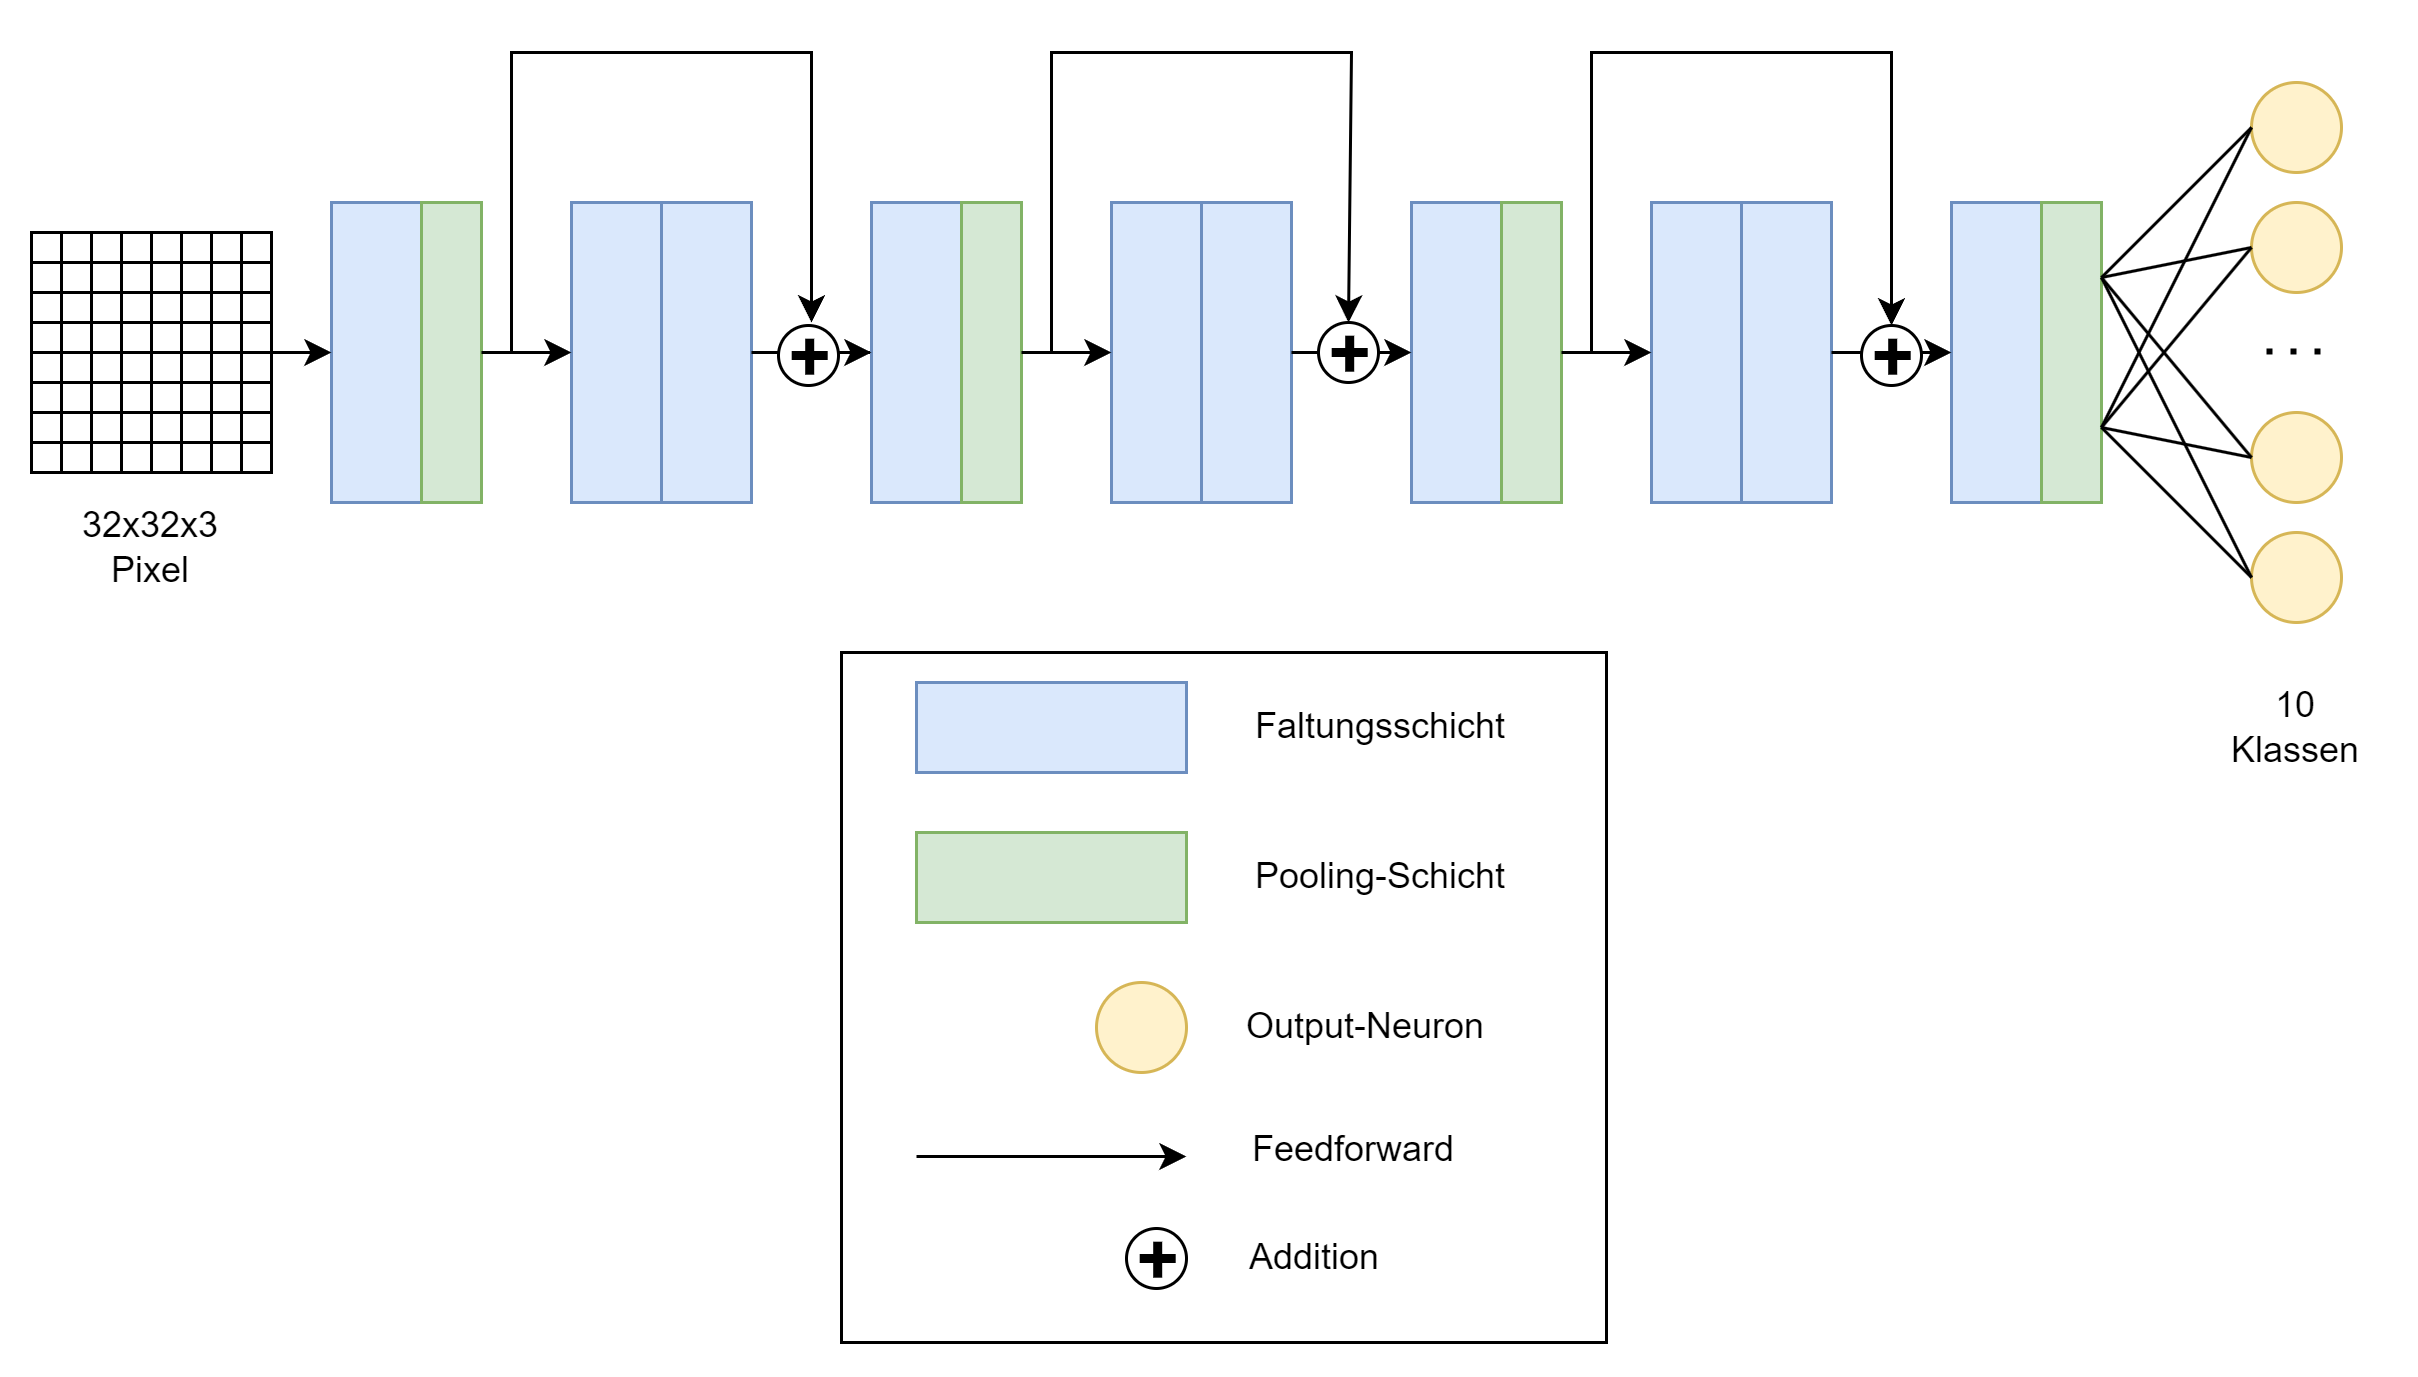
\includegraphics[width=15cm]{figures/cifar_modell.png}
    \caption{Neuronales Netz zur Klassifikation von CIFAR-10}
    \label{fig:cifar_modell}
\end{figure} 

Neben CIFAR-10, wird der CelebA Datenbestand \cite{celeba} genutzt, welcher unter anderem über die Plattform Kaggle zur Verfügung steht.
Dieser enthält 202.599 Bilder, auf welchen jeweils das Gesicht einer Person des öffentlichen Lebens zu sehen ist.
Die Bilder haben jeweils eine Auflösung von $178\times218$ Pixeln mit je 3 Farbkanälen.
Zu jedem Bild gibt es 40 Labels, wobei jedes davon eine Eigenschaft beschreibt. 
Dabei können jeweils die Werte -1 (Eigenschaft nicht vorhanden) und 1 (Eigenschaft vorhanden) angenommen werden.
Ein Beispiel für eine Eigenschaft ist die Größe eines Organs sein (Label \dq \textit{Big\_Nose}\dq).
Manche Eigenschaften können sich außerdem gegenseitig ausschließen.
So gibt es beispielsweise mehrere Labels für Haarfarben (Label \dq \textit{Black\_Hair}\dq\ und Label \dq \textit{Blond\_Hair}\dq).
Der Datenbestand ist bereits unterteilt in \dq \textit{Training}\dq, \dq \textit{Validierung}\dq\ und \dq \textit{Test}\dq.
Die vorgegebene Einteilung wird beibehalten, sodass die Güte des Modells immer auf der Testdatenmenge, welche nicht im Training genutzt werden, gemessen wird.
Tabelle \ref{tab:anzahl_datensaetze} zeigt die Anzahl der Datensätze in den jeweiligen Teildatenbeständen.

\begin{table}[!htb]
\centering
\begin{tabular}{|l|l|l|}
\hline
\rowcolor[HTML]{CBCEFB} 
{\color[HTML]{000000} Datenbestand} & Anzahl Datensätze  & prozentualer Anteil\\ \hline
Training & 162.770  &     $\approx$ 80\%  \\ \hline
Validierung & 19.867 &     $\approx$ 10\%      \\ \hline
Test  & 19.962 &    $\approx$ 10\%    \\ \hline

\end{tabular}
\caption{Anzahl Datensätze}
\label{tab:anzahl_datensaetze}
\end{table}

Der Use Case ist es dabei, alle 40 Label eines Bildes vorherzusagen.
Dabei handelt es sich um ein sogenanntes Multi-Label Klassifizierung, also eine Klassifikation bei der mehrere Klassen (hier Eigenschaften) bestimmt werden können.
Als Metrik zur Messung der Güte eines Modells wird dabei die Genauigkeit genutzt, also das Verhältnis von richtig vorhergesagten Labels zu der gesamten Anzahl an Labels.

Für diesen Use Case werden zwei unterschiedliche Modelle genutzt.
Bei dem ersten Modell handelt es sich um ein ResNet-18 Modell \cite{resnet}.
Dieses hat eine ähnliche Architektur wie das bereits beschriebene Modell für die Klassifizierung der CIFAR-10 Daten.
Jedoch besitzt dieses Modell 18 Faltungsschichten, wodurch die Anzahl der Parameter größer ist.
Das zweite Modell ist das sogenannte Vision Transformer Modell \cite{vit}, kurz ViT. 
Dieses Modell nutzt einige Elemente der Transformer-Architektur, welche ursprünglich aus dem Bereich der Computerlinguistik stammt \cite{transformer}. 
Das Vision Transformer Modell unterteilt das Bild in mehrere, gleich große Teilbilder, welche Patches genannt werden.
Dabei erhalten die Patches eine Position, welche von oben links nach unten rechts inkrementiert wird.
Die Patches werden über sogenannte Embedding-Schichten in einen höherdimensionalen Vektorraum übertragen.
Die entstandenen Vektoren werden Embeddings genannt.
Im Laufe des Trainingsprozesses, werden die Parameter der Embedding-Schichten so angepasst, dass die Ähnlichkeit zweier Embeddings mit der Ähnlichkeit der Eingabebilder korreliert. 
Die Embeddings werden anschließend mit der Position der jeweiligen Patches als Eingabe für einen oder mehrere sequentiell verbundene Kodierer, auch Encoder genannt, genutzt.
Diese bestehen aus jeweils mindestens einem Aufmerksamkeitsmechanismus, auch Attention genannt, und einigen vollständig verbundenen Schichten eines neuronalen Netzes.
Die Aufmerksamkeitsmechanismen erlernen verschiedene Beziehungen der Patches zueinander, welche durch die jeweiligen Positionen in einer räumlichen Verbindung stehen.
Die Ausgabe des letzten Kodierers wird anschließend als Eingabe für vollständig verbundene Schichten genutzt, welche die Klassifikation durchführen.
Neuronen der letzten Schicht repräsentieren jeweils eine Klasse.
\section{Wahl des Frameworks}

Viele der Methoden aus Kapitel \ref{ch:methoden} besitzen ein öffentliches Repository, in denen exemplarisch ein Beispiel umgesetzt und evaluiert wird.
Einige dieser Repositories sind seit Jahren nicht mehr gepflegt, weshalb die Wahl der entsprechenden Bibliotheken entscheidend sein kann.
Bei kryptografischen Methoden empfiehlt sich der Einsatz von bewährten, erforschten und gepflegten Bibliotheken.
Für Homomorphe Verschlüsselung gibt es beispielsweise die SEAL Bibliothek \cite{SEAL}, welche von Microsoft entwickelt wird, oder auch die HElib \cite{helib}.
Diverse Secure Multi-Party Computation Methoden, wie Yao's Garbled Circuits, werden in einer Bibliothek namens MP-SPDZ \cite{mp-spdz} implementiert.
Allerdings sind Bibliotheken für funktionale Verschlüsselung weniger gepflegt. So hat die Bibliothek CiFEr \cite{cifer} seit mehr als zwei Jahren keine Aktualisierung erhalten.

Um Differential Privacy zu nutzen, ist nicht zwingend eine spezialisierte Bibliothek notwendig. 
Die populäre Python Bibliothek NumPy \cite{numpy}, die in vielen Machine Learning Projekten eingesetzt wird, bietet bereits Funktionalität, um beispielsweise Werte mittels einer Laplace-Verteilung oder Gauß-Verteilung zu verrauschen.
Lediglich die Berechnung des Privacy Budgets fehlt in NumPy.

Die größten Frameworks für die Entwicklung von neuronalen Netzen sind PyTorch \cite{pytorch}, TensorFlow \cite{tensorflow} und JAX \cite{jax}. 
Tabelle \ref{tab:framworks} zeigt die Anzahl der Modelle, die jeweils mit dem entsprechenden Framework trainiert wurden und auf Hugging Face, einer Plattform zum Teilen von neuronalen Netzen, hochgeladen wurden \cite{HuggingFace}.
Das Framework PyTorch wurde dabei für fast 7 Mal so viele Modelle genutzt, wie die anderen beiden Frameworks zusammen.
\begin{table}[!htb]
\centering
\begin{tabular}{|l|l|}
\hline
\rowcolor[HTML]{CBCEFB} 
{\color[HTML]{000000} Framework} & Anzahl Modelle auf Hugging Face     \\ \hline
PyTorch & 122.061          \\ \hline
TensorFlow & 9.326             \\ \hline
JAX  & 8.560          \\ \hline

\end{tabular}
\caption{Anzahl Modelle je Framework auf Hugging Face \cite{HuggingFace}}
\label{tab:framworks}
\end{table}

PyTorch und TensorFlow besitzen beide ein offizielles Modul, welches den Einsatz von Differential Privacy während des Trainings eines neuronalen Netzes ermöglicht. 
Diese heißen Opacus \cite{opacus} und TensorFlow Privacy \cite{Tensorflowprivacy}.
Für das Framework JAX gibt es keine offizielle Erweiterung für Differential Privacy, lediglich ein paar Open-Source-Bibliotheken wie JAX-Privacy \cite{jaxprivacy}.
Für die nachfolgenden Experimente wird das Framework PyTorch mit der Erweiterung Opacus genutzt.
\section{Technische Implementierung von DPSGD}\label{sec:opacu_implementierung}
Opacus ist eine Bibliothek, welches das Framework PyTorch erweitert, indem das Training eines neuronalen Netzes mittels DPSGD ermöglicht wird \cite{opacus}.
Der Großteil des PyTorch Codes bleibt dabei unverändert, wird jedoch um einige Wrapper-Klassen der Opacus Bibliothek erweitert.

\begin{lstlisting}[language=Python,caption={Training einer Epoche in PyTorch},captionpos=b,showstringspaces=false,label={lst:torch_default}]
import torch

model:torch.nn.Module = <...> 
criterion:torch.nn.Module._Loss = torch.nn.CrossEntropyLoss()
optimizer:torch.optim.Optimizer = torch.optim.Adam(model.parameters(), 
                                                   lr=0.01)
train_dataloader:torch.utils.data.DataLoader = <...> 

for epoch in range(10):
    for inputs, labels in train_dataloader:
        optimizer.zero_grad()
        model_outputs = model(inputs)
        loss = criterion(model_outputs, labels)
        loss.backward()
        optimizer.step()
\end{lstlisting}

Listing \ref{lst:torch_default} zeigt die wichtigsten Komponenten beim Training eines neuronalen Netzes mit PyTorch.
Die Zeilen 3 bis 7 definieren die Objekte, die für das Training genutzt werden. 
Das Modell, welches trainiert werden soll, ist dabei vom Datentyp \textbf{torch.nn.Module} und wird in Zeile 3 als Platzhalter definiert.
Zeile 4 definiert die Verlustfunktion, welche in diesem Beispiel \textbf{torch.nn.CrossEntropyLoss} ist.
Als \textbf{Optimizer} wird \textbf{torch.optim.Adam} in Zeile 5 und 6 deklariert.
Bei einem \textbf{Dataloader} handelt es sich um ein Objekt, welches Batches von Datensätzen und die zugehörigen Labels über einen Iterator ausgibt.
Die Zeilen 10 bis 15 trainieren eine Epoche. 
Dabei wird jeder Batch, welche von dem \textbf{Dataloader} in Zeile 10 stammen, durch das Modell inferiert (Zeile 12). 
Mittels der Verlustfunktion werden die Gradienten der einzelnen Gewichte bestimmt (Zeile 13 und 14).
Der \textbf{Optimizer} passt anschließend die Gewichte in die entgegengesetzte Richtung der Gradienten, skaliert mit der Lernrate, an (Zeile 15).
Das Einbetten der Trainingslogik in eine For-Schleife ermöglicht das Training mehrerer Epochen hintereinander.

Opacus bietet Wrapper-Klassen, welche die Nutzung von DPSGD ermöglicht. 
Listing \ref{lst:opacus_pe1} zeigt, wie diese genutzt werden.
Zuerst wird ein Objekt des Typs \textbf{PrivacyEngine} in Zeile 3 deklariert.
Der Parameter \dq \textit{rdp}\dq \ als \dq \textit{accountant}\dq \ sorgt dafür, dass die Moments Berechnung aus Kapitel \ref{sec:dp_training} verwendet wird.
Die \textit{make\_private()}-Methode der \textbf{PrivacyEngine} akzeptiert das \textbf{Modell}, den \textbf{Optimizer} und den \textbf{Dataloader} und gibt diese jeweils in einer Wrapper-Klasse zurück.
Das Modell ist anschließend vom Datentyp \textbf{GradSampleModule\mbox} der Opacus Bibliothek. 
Normale PyTorch Modelle, vom Typ \textbf{torch.nn.Module\mbox}, berechnen aggregiert die Gradienten pro Batch, wohingegen die Wrapper-Klasse von Opacus\mbox, \textbf{GradSampleModule\mbox}, für jeden Datensatz eines Batches die Gradienten berechnet.
Grund dafür ist, dass die einzelnen Gradienten für das Clipping und das Verrauschen benötigt werden \cite{P-28}.
Das Clipping und Verrauschen übernimmt jedoch die Wrapper-Klasse des Optimizers. 
Diese ist vom Datentyp \textbf{DPOptimizer} der Opacus Bibliothek.
Der PyTorch \textbf{Dataloader\mbox} wird zu einem Opacus \textbf{DPDataloader} transformiert, welcher anschließend Batches mittels des Poisson-Samplings zusammenstellt.
Die \textit{make\_private()}-Methode benötigt noch zwei weitere Parameter: \textit{max\_grad\_norm} und \textit{noise\_multiplier}. 
Bei dem Wert von \textit{max\_grad\_norm} handelt es sich um die maximale Größe eines Gradienten, welche durch das Clipping beschränkt wird.
Der \textit{noise\_multiplier} definiert dabei die Stärke des Rauschens.
Diese wird mit der \textit{max\_grad\_norm} multipliziert und anschließend als Standardabweichung $\sigma$ des Gauß-Mechanismus, welcher für das Verrauschen der Gradienten zuständig ist, genutzt.

\begin{lstlisting}[language=Python,caption={Opacus Wrapper für DPSGD},captionpos=b,showstringspaces=false,label={lst:opacus_pe1}]
import opacus

privacy_engine = opacus.PrivacyEngine(accountant="rdp")
model, optimizer, data_loader = privacy_engine.make_private(
    module=model,
    optimizer=optimizer,
    data_loader=data_loader,
    noise_multiplier=1.0,
    max_grad_norm=1.0
)
#Hinterher normales Training des Modells
\end{lstlisting}

Nachdem die \textit{make\_private()}-Methode aufgerufen wurde und die entsprechenden Objekte von Opacus in Wrapper-Klassen umgewandelt wurden, wird das Modell mit gewöhnlichen PyTorch Code (Listing \ref{lst:torch_default}) trainiert. 
Um den $\epsilon$-Wert des Privacy Budgets zu begrenzen, kann nach jedem Training eines Batches oder einer Epoche der aktuelle $\epsilon$-Wert abgefragt werden und beim Überschreiten eines Grenzwerts das Training vorzeitig beendet werden.
Listing \ref{lst:calc_epsilon} zeigt den entsprechenden Methodenaufruf.
Dabei wird der $\delta$-Wert des Privacy Budgets als Parameter mitgegeben. 
Dieser wird im Voraus definiert und sollte kleiner als die Inverse der Anzahl an Datensätzen des Trainingsdatenbestands sein.

\begin{lstlisting}[language=Python,caption={Berechnung von Epsilon},captionpos=b,showstringspaces=false,label={lst:calc_epsilon}]
privacy_engine.accountant.get_epsilon(delta=1e-5)
\end{lstlisting}

Ein Nachteil der Nutzung der \textit{make\_private()}-Methode besteht darin, dass ein Wert für das Rauschen im Voraus festgelegt werden muss.
Bei einer zufälligen Wahl dieses Werts, ist unklar, wie viele Epochen trainiert werden können, bevor ein gewisses Privacy Budget überschritten wird. 
Um dieses Problem zu umgehen, kann als Alternative die Methode \textit{make\_private\_with\_epsilon()\mbox} genutzt werden.
Diese ist in Listing \ref{lst:opacus_pe2} zu sehen.
Anstatt dass hier eine Stärke des Rauschens übergeben wird, werden die gewünschte Anzahl an Epochen sowie das gewünschte Privacy Budget angegeben.
Anschließend berechnet Opacus die Stärke des Rauschens, sodass in etwa nach der festgelegten Anzahl an Epochen das Privacy Budget erreicht ist.
Jedoch kann der Wert des Privacy Budgets leicht abweichen. 
Dies liegt daran, dass durch das Poisson-Sampling die Anzahl an Datensätzen je Batch abweichen kann. 
Dadurch werden unterschiedlich viele Gradienten in jeder Epoche verrauscht.
Die Abweichung ist deshalb bei einer kleinen Anzahl an Epochen am größten.
Im Durchschnitt sollte die Größe der Batches jedoch der konfigurierten Batch-Größe entsprechen, sodass sich diese Abweichung über mehrere Epochen hinweg ausgleicht.


\begin{lstlisting}[language=Python,caption={Opacus Wrapper mit definiertem Epsilon},captionpos=b,showstringspaces=false,label={lst:opacus_pe2}]
import opacus

privacy_engine = opacus.PrivacyEngine(accountant="rdp")
model, optimizer, data_loader = privacy_engine.make_private_with_epsilon(
    module=model,
    optimizer=optimizer,
    data_loader=data_loader,
    epochs=10,
    target_epsilon=10,
    target_delta=1e-5,
    max_grad_norm=1.0
)
#Hinterher normales Training des Modells
\end{lstlisting}



\subsubsection*{Einschränkungen der Modellarchitektur}

Nicht jede Schicht eines Modells wird von DPSGD unterstützt und kann deshalb genutzt werden. 
Opacus bietet eine Klasse \textbf{ModuleValidator\mbox} an, welche überprüft, ob ein Modell kompatibel ist und bei Bedarf inkompatible Schichten austauscht.
Listing \ref{lst:modulevalidator} zeigt, wie diese Klasse genutzt werden kann.
Die \textit{validate()}-Methode aus Zeile 1 gibt dabei lediglich eine Liste mit inkompatiblen Schichten, sowie jeweils einer kurzen Erklärung dazu, zurück.
Um die inkompatiblen Schichten mit kompatiblen, alternativen Schichten ausgetauscht werden, kann die \textit{fix()}-Methode aufgerufen werden. 
\begin{lstlisting}[language=Python,caption={Opacus ModuleValidator} ,captionpos=b,showstringspaces=false,label={lst:modulevalidator}]
incompatible_layers = opacus.validators.ModuleValidator.validate(model)
model = opacus.validators.ModuleValidator.fix(model)
\end{lstlisting}

Ein Beispiel für eine nicht kompatible Schicht ist die sogenannte \textbf{BatchNorm}-Schicht.
Diese Schicht berechnet Mittelwerte und Standardabweichung über mehrere Datensätze eines Batches und nutzt diese anschließend für die Normalisierung der Datensätze.
Folglich wird ein Datensatz durch andere Datensätze in dem gleichen Batch beeinflusst, was jedoch nicht gewünscht ist. 
Dies liegt daran, dass laut DPSGD (Kapitel \ref{sec:dp_training}) ein Datensatz ($\epsilon$,$\delta$)-Differential Privacy in Bezug auf einen Batch erfüllen soll \cite{P-28}.
Alternative Schichten sind die \textbf{LayerNorm}-Schicht, die \textbf{InstanceNorm}-Schicht oder die \textbf{GroupNorm}-Schicht.
All diese Schichten dienen ebenfalls der Normalisierung, jedoch nicht anhand anderer Datensätze eines Batches \cite{opacus_blog_part3}.

\subsubsection*{Laufzeit und Speicherverbrauch}
Wie bereits erwähnt, berechnen normale PyTorch Modelle die Gradienten der Gewichte aggregiert über einen Batch.
Der Grund dafür ist die Performance, denn die Berechnung von Gradienten einzelner Datensätze, ist beim Training ohne Differential Privacy nicht nötig. 
DPSGD benötigt jedoch genau diese Gradienten einzelner Datensätze, um diese per Clipping und Verrauschen zu verändern \cite{P-28}, weshalb diese in Opacus berechnet werden \cite{opacus}.
Jedoch sorgt dies für eine längere Laufzeit, sowie einen erhöhten Speicherverbrauch.

Der Faktor, um welchen sich die Laufzeit erhöht, hängt dabei primär von den Arten der Schichten eines neuronalen Netzes ab. 
Faltungsschichten, Normalisierungsschichten und sogenannte Multi-Head-Attention-Schichten sorgen für eine Erhöhung der Laufzeit um den Faktor 1,2 bis 2,9.
Bei vollständig verbundenen Schichten und den sogenannten Embedding-Schichten\mbox, skaliert der Faktor der Laufzeit mit der Batch-Größe \cite{opacus}.
Der Speicherverbrauch skaliert ebenfalls mit der Batch-Größe.
Dies liegt daran, dass für jedes Gewicht nicht nur ein Gradient im Speicher gehalten wird, sondern jeweils ein Gradient für jeden Datensatz eines Batches \cite{opacus}.

Das Poisson-Sampling von DPSGD sorgt dafür, dass die tatsächliche Batch-Größe von der festgelegten Batch-Größe abweichen kann. 
Dies kann jedoch zu einem Problem werden, wenn die festgelegte Batch-Größe so ausgewählt wurde, dass der zur Verfügung stehende Speicher der GPU nahezu vollständig ausgenutzt wird.
Weicht die Batch-Größe nach oben ab, hat also mehr Datensätze als festgelegt, kann es sein, dass der Speicher nicht ausreicht und eine sogenannte \textbf{OutOfMemoryException} geworfen wird.
Dies sorgt für einen Abbruch des Trainings, woraufhin der Speicher geleert werden müsste und das Training neu gestartet werden müsste.
Um dies zu verhindert, bietet Opacus eine Lösung in Form der Klasse \textbf{BatchMemoryManager} an.
Diese Klasse wrappt den Dataloader nochmals in eine Wrapper-Klasse, bei welcher ein Parameter \dq \textit{max\_physical\_batch\_size}\dq\ mitgegeben wird. 
Der neue, zurückgegebene Dataloader beschränkt die tatsächliche Batch-Größe auf die als Maximum festgelegte Batch-Größe, sodass ein Überlaufen des Speichers verhindert wird.
Listing \ref{lst:memory_manager} zeigt, wie der BatchMemoryManager in den Trainingsprozess integriert wird.
Außerdem kann dieser auch genutzt werden, um mit virtuellen Batches zu trainieren. 
Dabei kann die Batch-Größe des Dataloaders höher konfiguriert werden, als die maximale Batch-Größe des BatchMemoryManagers. 
Dies sorgt dafür, dass die einzelnen Gradienten jeden Datensatzes anhand der kleineren Batches des BatchMemoryManagers berechnet werden.
Jedoch erfolgt die Aggregierung der Gradienten und das Anpassen der Gewichte erst, wenn die konfigurierte Batch-Größe des Dataloaders erreicht wurde.

\begin{lstlisting}[language=Python,caption={Opacus BatchMemoryManager},captionpos=b,showstringspaces=false,label={lst:memory_manager}]
with BatchMemoryManager( 
    data_loader=train_dataloader,
    max_physical_batch_size=64,
    optimizer=optimizer) 
as memory_safe_data_loader:
        for model_inputs,labels in mmemory_safe_data_loader:
            # Training ...
\end{lstlisting}

Tabelle \ref{tab:memory} zeigt, wie hoch der Speicherverbrauch bei den bereits beschriebenen Use Cases ist. 
Dabei wird der Speicher der Grafikkarte, auch VRAM genannt, betrachtet, da dieser oftmals ein limitierender Faktor ist.
Für das CIFAR-10 Modell, welches eine ResNet-Architektur nutzt, steigt der Speicherverbrauch bei der Nutzung von DPSGD mit Opacus um den Faktor 1,8 bis 5,0.
Für beide Modelle, welche Merkmale aus Gesichtern erkennen, wurde jeweils nur eine Batch-Größe betrachtet.
Dabei ist die Batch-Größe eine Zweierpotenz, die so gewählt ist, dass der entsprechende Batch mit DPSGD und Opacus noch in den Speicher passt. 
Der maximale Speicher der genutzten Hardware liegt bei 24 GB VRAM (siehe Anhang \ref{ch:hard_software}).
Der Speicherverbrauch des ResNet-18-Modells steigt um den Faktor 2,8 bei einer Batch-Größe von 64.
Für das Vision Transformer Modell kann jedoch nur eine Batch-Größe von 16 ausgewählt werden, da hier mit 20,8 GB Speicherauslastung fast das Limit der Hardware erreicht ist.
Die relativ geringe Batch-Größe sorgt lediglich für eine Differenz von 1,6 Mal so viel Speicherauslastung, wie ohne DPSGD.
\begin{table}[!htb]
\centering
\begin{tabular}{|l|l|l|l|l|}
\hline
\rowcolor[HTML]{CBCEFB} 
Modell                   & Batch-Größe & \begin{tabular}[c]{@{}l@{}}Speicherverbrauch\\ ohne DPSGD\end{tabular} & \begin{tabular}[c]{@{}l@{}}Speicherverbrauch\\ mit DPSGD\end{tabular} & \begin{tabular}[c]{@{}l@{}}Faktor \\ Differenz\end{tabular} \\ \hline
CIFAR-10 Modell          & 64          & 2,8 GB VRAM                                                         & 5,1 GB VRAM                                                         & 1,8                                                         \\ \hline
CIFAR-10 Modell          & 128         & 2,9 GB VRAM                                                          & 10,2 GB VRAM                                                        & 3,5                                                         \\ \hline
CIFAR-10 Modell          & 256         & 3,3 GB VRAM                                                          & 16,4 GB VRAM                                                        & 5,0                                                           \\ \hline
CelebA ResNet-18          & 64          & 4,6 GB VRAM                                                          & 12,8 GB VRAM                                                        & 2,8                                                         \\ \hline
CelebA ViT & 16          & 12,8 GB VRAM                                                         & 20,8 GB VRAM                                                        & 1,6                                                         \\ \hline
\end{tabular}
\caption{Speicherverbrauch mit und ohne Differential Privacy}
\label{tab:memory}
\end{table}

Tabelle \ref{tab:memory} zeigt, wie die Trainingsdauer einer Epoche für die Modelle variieren kann.
Dabei wurden die gleichen Batch-Größen gewählt, wie bei der Messung des Speicherverbrauchs.
Die Trainingsdauer des CIFAR-10 Modells erhöht sich um einen Faktor von 1,3 bis 3,1.
Da eine Epoche jedoch nur wenige Sekunden benötigt, fällt die absolute Differenz relativ gering aus.
Die Modelle der Merkmalserkennung sind demgegenüber komplexer und benötigen ohne DPSGD bereits mehrere Minuten für das Training einer Epoche. 
Jedoch erhöht sich der Faktor hier auf 4,5 oder 10,0. 
Dies liegt zum einen an den Arten der Schichten und zum anderen an einem Softwarefehler des Frameworks.
Das ResNet-18-Modell nutzt einige Normalisierungsschichten, das Vision Transformer Modell nutzt einige Multi-Head-Attention Schichten für die Implementierung eines Aufmerksamkeitsmechanismus.
Die zusätzliche Laufzeit dieser Schichten, skaliert bei Opacus mit der Batch-Größe, wodurch hier ein höherer Multiplikationsfaktor entstehen kann.
Zusätzlich gibt es einen Softwarefehler des Dataloaders in Kombination mit Opacus, welcher dazu führt, dass das Laden von Daten nur in einem Thread ausgeführt werden kann und nicht zeitgleich in mehreren.
Der Fehler wird im folgenden genauer beleuchtet.
Der gleiche Fehler existiert auch bei den CIFAR-10 Modellen, fällt da jedoch weniger ins Gewicht, da das Laden der Bilder aufgrund der geringeren Auflösung weniger Zeit benötigt.
\begin{table}[!htb]
\centering
\begin{tabular}{|l|l|l|l|l|}
\hline
\rowcolor[HTML]{CBCEFB} 
Modell                    & Batch-Größe & \begin{tabular}[c]{@{}l@{}}Dauer Epoche\\ ohne DPSGD\end{tabular} & \begin{tabular}[c]{@{}l@{}}Dauer Epoche\\ mit DPSGD\end{tabular} & \begin{tabular}[c]{@{}l@{}}Faktor \\ Differenz\end{tabular} \\ \hline
CIFAR-10 Modell           & 64          & 7 Sekunden                                                     & 22 Sekunden                                                   & 3,1              \\ \hline
CIFAR-10 Modell           & 128         & 7 Sekunden                                                     & 18 Sekunden                                                   & 2,6              \\ \hline
CIFAR-10 Modell           & 256         & 14 Sekunden                                                    & 18 Sekunden                                                   & 1,3              \\ \hline
CelebA ResNet-18           & 64          & 3 Minuten                                                      & 30 Minuten                                                    & 10,0               \\ \hline
CelebA ViT & 16          & 11 Minuten                                                     & 50 Minuten                                                    & 4,5              \\ \hline
\end{tabular}
\caption{Dauer des Trainings einer Epoche mit und ohne Differential Privacy}
\label{tab:dauer_epoch}
\end{table}

\subsubsection*{Softwarefehler}

Da Opacus eine optionale Erweiterung von PyTorch ist, ist die Bibliothek weniger genutzt.
Dies ist über die Statistiken von GitHub erkennbar. 
Während es auf GitHub fast 304.000 Repositories gibt, die PyTorch benutzen\footnote{https://github.com/pytorch/pytorch}, sind es bei Opacus lediglich knapp 600\footnote{https://github.com/pytorch/opacus}.
Laut diesen Zahlen, nutzen nur \ca 0,2 \% der Projekte mit PyTorch zusätzlich noch Opacus.
Dies kann ein Grund sein, warum deutlich weniger Ressourcen in die Entwicklung von Opacus fließen.
Bei PyTorch haben fast 3000 Personen über GitHub etwas zur Entwicklung des Frameworks beigetragen, wohingegen bei Opacus lediglich 55 Personen beteiligt waren.
Dies könnte ein Grund sein, warum Opacus einige Softwarefehler hat, oder warum einige Features nicht vollumfänglich funktionieren.

Ein Softwarefehler, der die Trainingsdauer der Epoche erhöht, entsteht bei der Parallelisierung des Dataloaders.
Der Dataloader kann über einen Parameter \dq\textit{num\_workers}\dq\ eine vorgegebene Anzahl an Threads starten. 
Jeder dieser Threads lädt dabei einen Batch an Datensätzen in den Speicher, sodass nach dem Training eines Batches bereits der nächste Batch zur Verfügung steht.
Durch die Wrapper-Klasse in Opacus, welche das Poisson-Sampling implementiert, ist diese Parallelisierung nicht mehr möglich.
Dies sorgt dafür, dass wenn die GPU einen Batch zum Training genutzt hat, es sein kann, dass der nächste Batch noch nicht geladen ist und somit die GPU auf diesen warten muss.
Je komplexer die Daten und die Prozesse des Ladens sind, desto länger dauert das Laden eines Batches.
Bei dem CelebA Datenbestand muss jedes Bild, welches jeweils eine Dimension von $178\times218\times3$ hat, von der Festplatte der Hardware geladen werden.
Dies ist der Grund, warum das CelebA ResNet-18-Modell mit DPSGD die 10-fache Trainingsdauer einer Epoche erreicht, als im Vergleich zum Training ohne DPSGD.

Ein Beispiel für ein Feature, welches nicht vollumfänglich funktioniert, ist die Nutzung eines adaptiven Werts für das Clipping.
Die Technik mit dem Namen AdaClip sorgt dafür, dass die Clipping-Norm variabel ist und sich den Gradienten anpasst \cite{adaclip}.
Dadurch könnte der Wert möglichst gering sein, was auch das hinzugefügte Rauschen verkleinern würde.
Die Klasse, welche die entsprechende Logik enthält, existiert in Opacus unter dem Namen \textbf{AdaClipDPOptimizer}.
Jedoch gibt es zwei Probleme, welche die Nutzung der Klasse erschweren oder nicht möglich machen.
Das erste Problem ist, dass die Übergabe der Parameter nicht korrekt funktioniert. 
Die \textit{make\_private()}-Methode kann über den Parameter \dq\textit{clipping}\dq\ mit dem Wert \dq\textit{adaptive}\dq\ so aufgerufen werden, dass der AdaClipDPOptimizer genutzt werden würde.
Jedoch braucht diese Klasse zusätzliche Parameter, welche nicht über die \textit{make\_private()}-Methode weitergegeben werden können.
Um dieses Problem zu umgehen, müssen die Wrapper-Klassen manuell konfiguriert werden.
Das zweite Problem liegt in der Klasse selber.
PyTorch hat einige Kontrollen integriert, welche sicherstellen sollen, dass das Training in einem vorgegebenen Rahmen ausgeführt wird. 
Eine dieser Kontrollen ist es, dass die Gradienten vor dem Training eines Batches zurückgesetzt werden, damit Gradienten nicht mehrfach genutzt werden.
Bei Nutzung der Klasse AdaClipDPOptimizer kommt es jedoch zu einem Fehler dieser Kontrolle.

Obwohl die Behebung diverser Fehler und das Hinzufügen fehlender Funktionalität große Relevanz hat, ist dies im Rahmen der Arbeit nicht möglich.
Deshalb werden mögliche Fehler umgangen.
Die nicht mögliche Parallelisierung des Dataloaders schränkt die Funktionalität nicht ein, sondern erhöht nur die Laufzeit. 
Im Gegensatz dazu, ist die Nutzung der adaptiven Clipping-Norm nicht ohne entsprechenden Aufwand möglich, weshalb im folgenden lediglich konstante, festgelegte Werte für das Clipping betrachtet werden.


\section{Hyperparameter von DPSGD}\label{sec:hyperparams}

Die Güte eines Modells wird durch die Wahl der Hyperparameter beeinflusst. 
Dies gilt sowohl beim normalen Training, als auch beim Training mit DPSGD.
Im Folgenden wird getestet, welche Parameter die Güte eines neuronalen Netzes bei der Nutzung von DPSGD beeinflussen.
Dazu werden die drei Modelle, welche in Kapitel \ref{sec:use_case} beschrieben wurden, mit verschiedenen Hyperparametern trainiert und evaluiert.
Dabei werden DPSGD spezifische Parameter, wie der $\epsilon$-Wert und die Clipping-Norm, und auch allgemeine Parameter, wie die Batch-Größe und die Anzahl der Epochen, betrachtet.
Die Lernrate wird dabei nicht konstant festgelegt, sondern über den \textbf{Adam}-Optimizer in PyTorch adaptiv konfiguriert.
Der Adam-Optimizer passt die Lernrate anhand des Momentums und der Varianz der Gradienten an \cite{adam}.

Bevor das eigentliche Modell trainiert wird, gibt es die Möglichkeit, die Datenmenge per Datenaugmentierung, auch Data Augmentation genannt, künstlich zu erweitern.
Bei Bildern können die Werte einzelner Pixeln beeinflusst werden, indem der Farbraum der Bilder angepasst wird, oder Kontraste erhöht werden.
Zusätzlich können Bilder über Rotation und Spieglung transformiert werden.
Dabei können die Werte der Anpassung, \zB die Verstärkung des Kontrasts, konfiguriert werden und an eine Wahrscheinlichkeit geknüpft werden.
PyTorch bietet über AutoAugment eine Möglichkeit an, eine Kombination verschiedener Anpassungen zu nutzen \cite{autoaugment}.
Die Nutzung von AutoAugment, sowie dessen Einfluss auf die Güte der Modelle, wird folglich mitberücksichtigt.

Da das CIFAR-10 Modell die geringste Anzahl an lernbaren Parameter besitzt, wird die Anpassung verschiedener Parameter an diesem Modell zuerst evaluiert.
Anschließend werden die Erkenntnisse auf das ResNet-18 Modell und das Vision Transformer Modell für den CelebA Datenbestand angewendet.
Im Folgenden werden einige Auszüge aus den gesamten Ergebnissen zur Veranschaulichung herangezogen. 
Die vollständigen Tabellen aller Messwerte befinden sich in Anhang \ref{ch:ergebnisse_detail}.

\subsection{Hyperparameter CIFAR-10 Modell}

Für das CIFAR-10 Modell, welches kein DPSGD nutzt, werden folgende Hyperparameter betrachtet: Anzahl der Epochen, Batch-Größe und die Nutzung von AutoAugment.
Dazu wurde das Modell mit einer Epochenanzahl zwischen 10 und 20 trainiert, jeweils mit einer Batch-Größe von 64, 128 oder 256. 
Dieser Vorgang wurde mit AutoAugment aktiviert und deaktiviert ausgeführt.
Die höchste Genauigkeit wird erreicht, wenn das Modell mit Datenugmentierung und einer Batch-Größe von 64 über 15 Epochen hinweg trainiert wird.
Die erreichte Genauigkeit, welche anhand der Test-Daten gemessen wurde, liegt bei 84,6 \%.

Eine Batch-Größe von 64 und 128 resultieren in einer ähnlichen Güte des Modells. 
Jedoch sorgt eine Batch-Größe von 256 für eine geringere Genauigkeit des Modells. 
Dies liegt daran, dass einzelne Datensätze in der Aggregation der Gradienten untergehen können, wodurch einzelne Features der Daten weniger gut gelernt werden. 
Abbildung \ref{fig:cifar-1} zeigt die Güte der Modelle, welche mit den unterschiedlichen Batch-Größen trainiert wurden.
Jede Linie steht dabei für eine unterschiedliche Anzahl an trainierten Epochen.
\begin{figure}[!htb]
    \centering
    \fbox{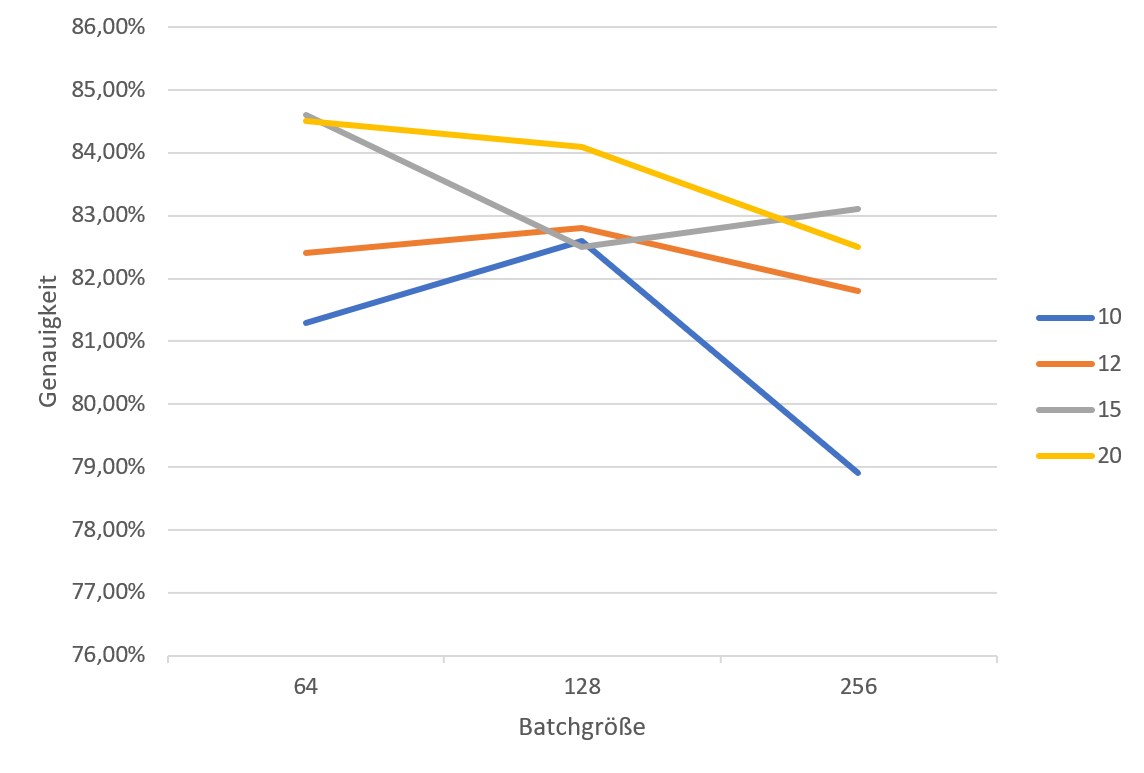
\includegraphics[width=14cm]{figures/results_cifar/cifar_batch_base.png}}
    \caption{Auswirkung Batch-Größe auf CIFAR-10 Modell ohne DPSGD und mit \\Datenaugmentierung}
    \label{fig:cifar-1}
\end{figure} 

Zusätzlich zeigt Abbildung \ref{fig:cifar-1}, dass eine höhere Anzahl an Epochen mit einer höheren Genauigkeit korreliert.
Dies liegt an der Nutzung von Datenaugmentierung. 
Wird diese nicht genutzt, liegt die optimale Anzahl an Epochen zwischen 12 und 15. 
Werden mehr Epochen trainiert, sinkt die Genauigkeit wieder, was auf ein Overfitting des Modells zurückzuführen ist.
Generell sinkt die Genauigkeit der Modelle, wenn AutoAugment nicht genutzt wird. 
Durch die Datenaugmentierung wird der Datensatz künstlich erweitert, was dafür sorgt, dass die Trainingsdatenmenge vergrößert wird.

Für das CIFAR-10 Modell ohne DPSGD resultieren folgendende Hyperparameter in einer optimalen Güte des Modells:
\begin{compactitem}
    \item \textbf{Batch-Größe:} Batch-Größe kann variablen gewählt werden, sollte jedoch nicht zu groß sein. Ein Wert von 64 oder 128 ist wirksam.
    \item \textbf{Anzahl Epochen:} Die optimale Anzahl an Epochen ist um 15 herum. Wird Datenaugmentierung genutzt, kann die Anzahl höher sein, wenn nicht, dann sollte die Anzahl geringer sein.
    \item \textbf{Datenaugmentierung:} Datenaugmentierung verbessert die Güte des Modells und ermöglicht das Training mehrerer Epochen, wobei Overfitting vermieden wird. Datenaugmentierung sollte deshalb genutzt werden.
\end{compactitem}


Wird das CIFAR-10 Modell mit DPSGD trainiert, müssen zusätzlich noch der $\epsilon$-Wert des Privacy Budgets und die Clipping-Norm betrachtet werden. 
Der $\delta$-Wert des Privacy Budgets wird konstant auf $10^{-5}$ festgelegt.
Um die Hyperparameter zu evaluieren, gibt es drei unterschiedliche Versuche.
Alle drei Versuche trainieren eine Vielzahl an Modellen mit DPSGD.
Dabei werden $\epsilon$-Werte von 1 bis 50, Epochenanzahlen von 1 bis 30 und Batch-Größen von 64 bis 256 genutzt.
Lediglich bei der Clipping-Norm und bei der Nutzung von Datenaugmentierung unterscheiden sich die drei Versuche.
Um den festgelegten $\epsilon$-Wert nach einer festgelegten Anzahl an Epochen zu erreichen, wurde die \textit{\mbox{make\_private\_with\_epsilon()}}-Methode genutzt.

Der erste Versuch nutzt Datenaugmentierung und hat einen nicht optimierten Wert der Clipping-Norm.
Dieser ist auf 1,0 festgelegt.
Dieser Versuch zeigt, dass die Genauigkeit der Modelle, mit der Größe des $\epsilon$-Werts zunimmt.
Bei einem $\epsilon$-Wert von 1 wird maximal eine Genauigkeit von 36,9 \% erreicht, wohingegen bei einem $\epsilon$-Wert von 50 eine Genauigkeit von 59,1 \% erreicht wird.
Ebenfalls steigt die Genauigkeit der Modelle mit der Anzahl an trainierten Epochen. 
Dies liegt daran nicht nur daran, dass Datenaugmentierung genutzt wird, sondern dass auch das Rauschen Overfitting verhindert.
Sogar 30 Epochen können trainiert werden, ohne dass die Genauigkeit stagniert.
Anders als bei dem Modell ohne DPSGD, hat die Batch-Größe eine deutliche Auswirkung auf die Genauigkeit der Modelle.
Eine höhere Batch-Größe sorgt für eine verbesserte Genauigkeit der Modelle.
Das Rauschen, welches den einzelnen Gradienten hinzugefügt wird, gleicht sich bei einer höheren Batch-Größe aus und nähert sich dem Erwartungswert an. 
Da der Erwartungswert den echten Gradienten entspricht, bedeutet dies, dass eine höhere Batch-Größe dafür sorgt, dass die verrauschten Gradienten der Gewichte, näher an den tatsächlichen Gradienten der Gewichte liegen.
Abbildung \ref{fig:cifar-2} zeigt diesen Zusammenhang grafisch.
Jede Linie entspricht einem Modell, welches über 15 Epochen, mit unterschiedlichem $\epsilon$-Wert, trainiert wird.
\begin{figure}[!htb]
    \centering
    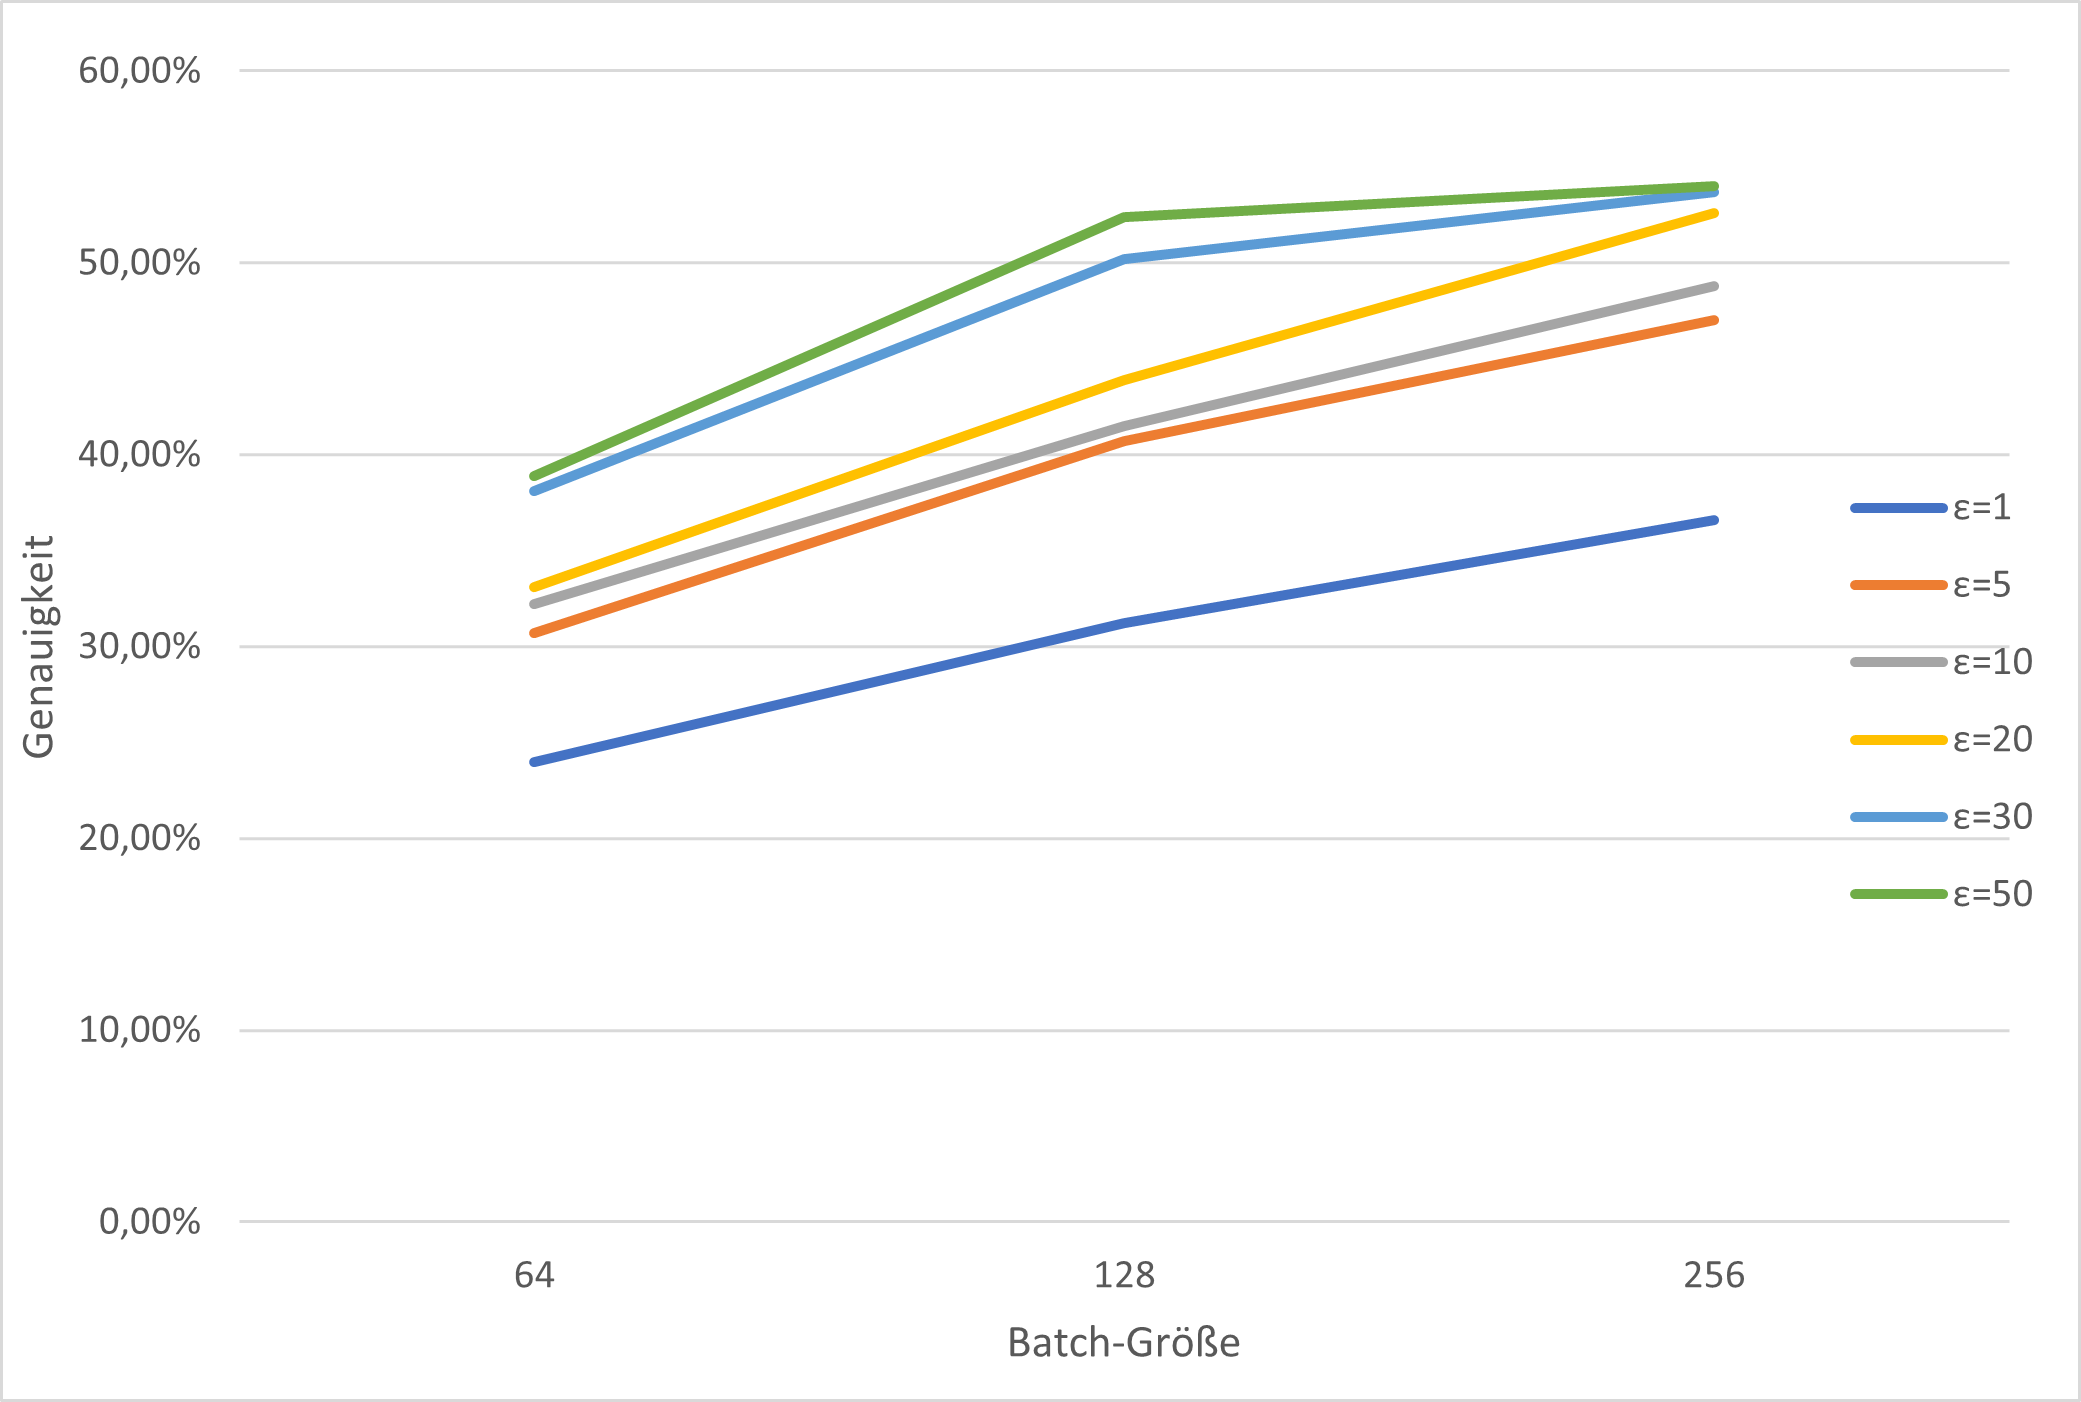
\includegraphics[width=14cm]{figures/results_cifar/cifar_batch_1.png}
    \caption{Auswirkung der Batch-Größe auf die Genauigkeit von CIFAR-10 Modellen}
    \label{fig:cifar-2}
\end{figure} 

Der zweite Versuch ähnelt dem ersten Versuch, jedoch wird die Datenaugmentierung nicht genutzt.
Dies sorgt dafür, dass die Genauigkeit der Modelle steigt. 
Abbildung \ref{fig:cifar_aug3} zeigt diesen Zusammenhang.
Die Modelle, dessen Genauigkeit dargestellt werden, werden jeweils 15 Epochen lang, mit einer Batch-Größe von 256, trainiert.
\begin{figure}[!htb]
    \centering
    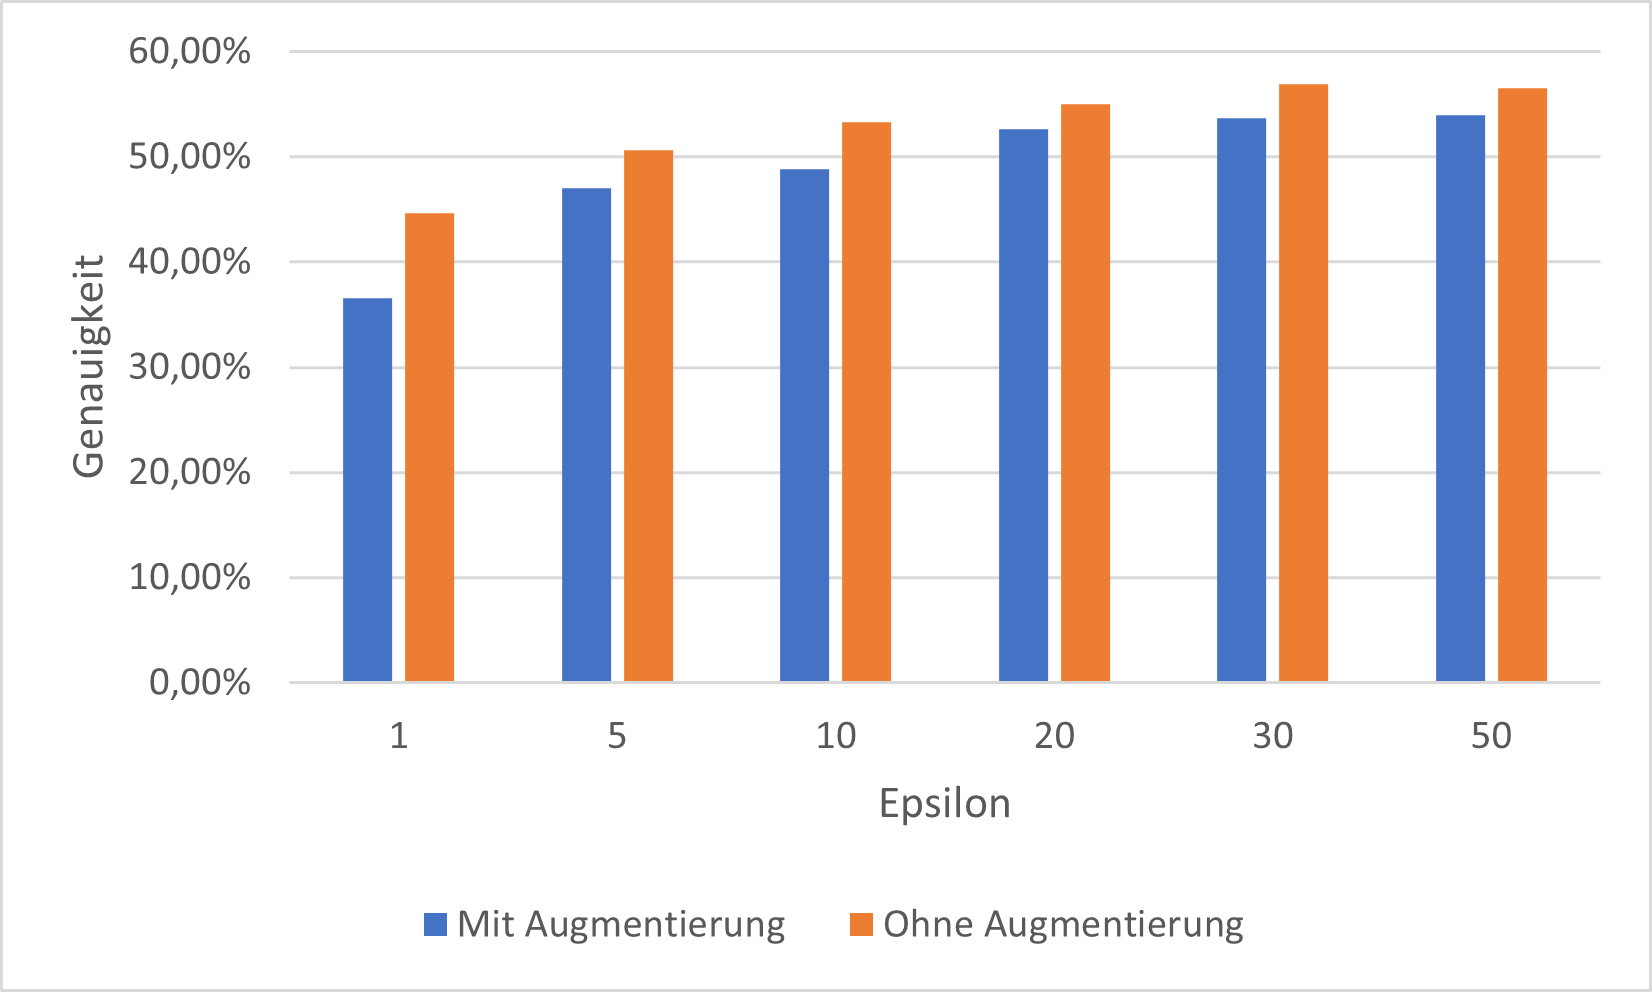
\includegraphics[width=14cm]{figures/results_cifar/cifar_aug3.png}
    \caption{Auswirkung von AutoAugment auf die Genauigkeit von CIFAR-10 Modellen}
    \label{fig:cifar_aug3}
\end{figure} 
Obwohl die Datenaugmentierung im zweiten Versuch nicht genutzt wird, kann das Modell 20 Epochen lang trainiert werden und hat dennoch eine steigende Genauigkeit.
Erst im Bereich zwischen 20 und 30 Epochen stagniert die Genauigkeit.
Im Vergleich zu dem Modell ohne DPSGD sind dies dennoch einige Epochen mehr.
Dies liegt daran, dass das Rauschen, genau wie die Datenaugmentierung, das Overfitting reduziert.

Der dritte Versuch gleicht dem zweiten Versuch, wobei hier der Wert der Clipping-Norm angepasst wurde.
Da die Clipping-Norm die Stärke des Rauschens beeinflusst, kann ein geringer Wert die Güte eines Modells erhöhen.
Wird der Wert jedoch zu gering gewählt, kann dies auch für den gegenteiligen Effekt sorgen, denn die Gradienten werden zu klein, damit das Modell in den geplanten Trainingsschritten konvergiert.
Um eine geeignete Clipping-Norm zu finden, wird das CIFAR-10 Modell über 5 Epochen trainiert, ohne Rauschen, jedoch mit unterschiedlichen Werten für das Clipping.
Dabei werden Zehnerpotenzen genutzt.
Der Wert wird immer um eine Zehnerpotenz reduziert, solange bis das Clipping einen leichten negativen Einfluss auf die Güte des Modells hat.
Die resultierende Zehnerpotenz ist in diesem Fall $10^{-5}$.
Da diese einen leichten negativen Einfluss auf das Modell hat, bedeutet dies, dass eine Vielzahl an Gradienten durch diesen Wert begrenzt wird.
Die Wahl der Clipping-Norm sollte auf diesen Wert fallen, oder einen minimal höheren Wert, welcher keinen Einfluss auf das Modell hat.
Durch die Wahl dieses geringen Werts wird auch die Stärke des Rauschens reduziert.
In diesem dritten Versuch wird die Clipping-Norm von $10^{-5}$ evaluiert.

Die Anpassung der Clipping-Norm wirkt sich nicht bei einer niedrigen Anzahl an Epochen aus.
Bei den CIFAR-10 Modellen, welche 15 Epochen lang trainiert werden, ist die Genauigkeit in etwa gleich, egal ob die Clipping-Norm bei 1 oder bei $10^{-5}$ liegt. 
Abbildung \ref{fig:cifar_clip1} zeigt den soeben beschriebenen Zusammenhang.
\begin{figure}[!htb]
    \centering
    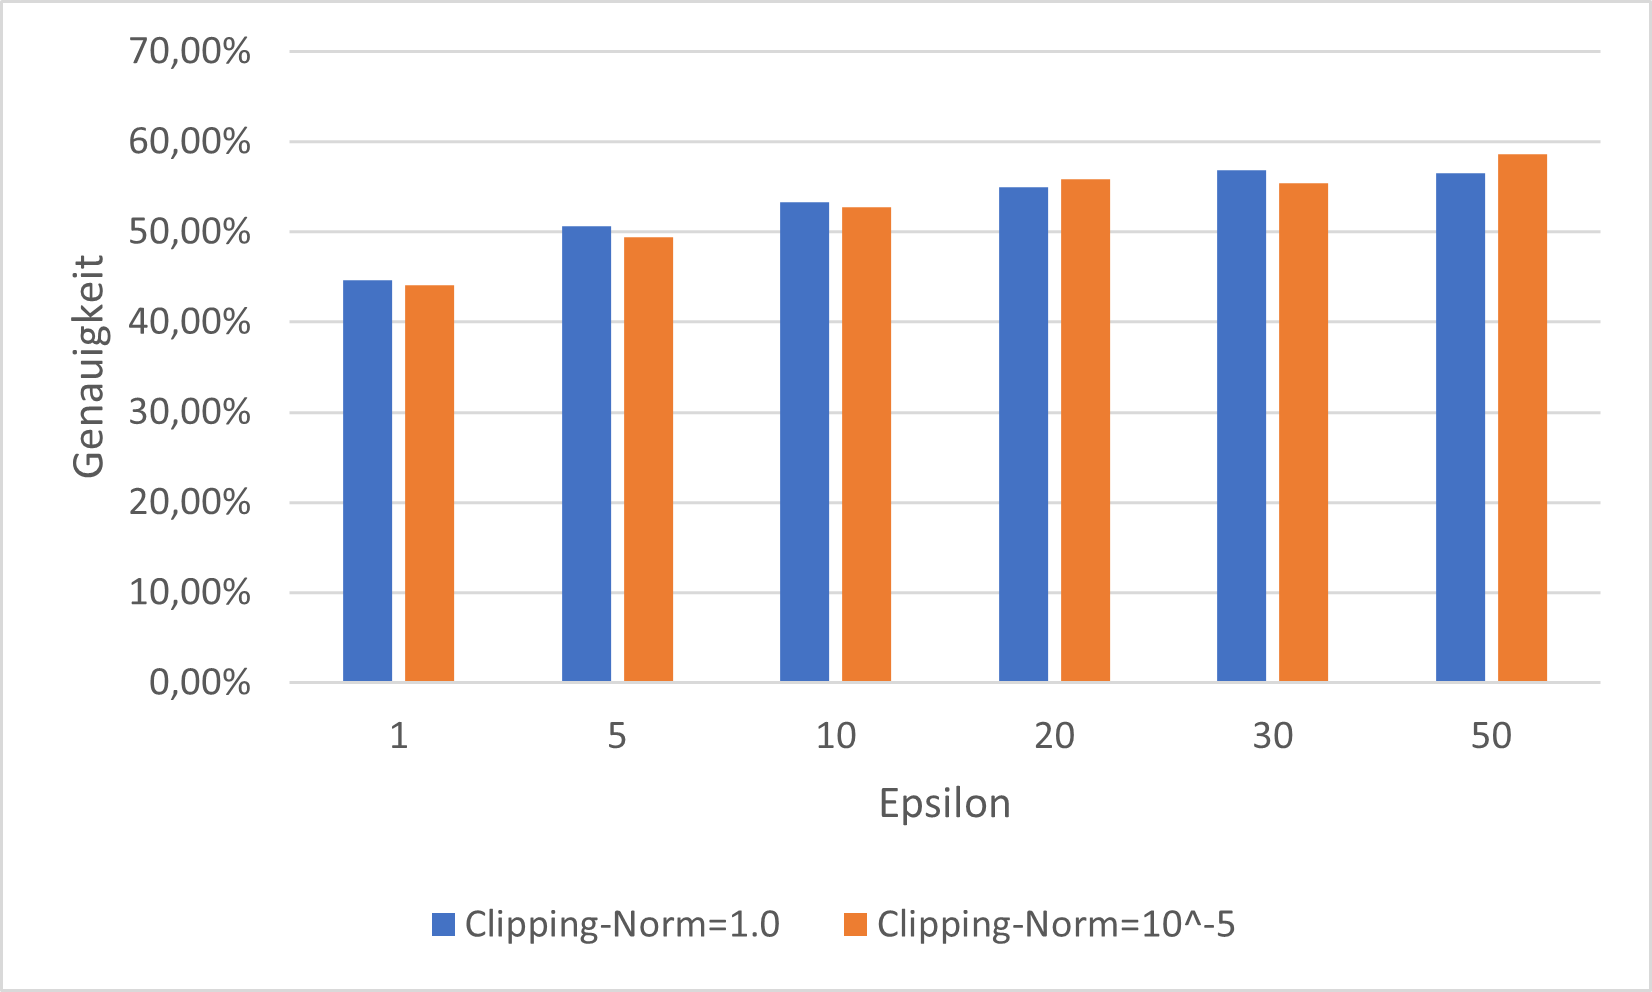
\includegraphics[width=14cm]{figures/results_cifar/cifar_clipp1.png}
    \caption{Auswirkung der Clipping-Norm auf die Güte von CIFAR-10 Modellen bei 15 Epochen Training}
    \label{fig:cifar_clip1}
\end{figure} 

Jedoch ermöglicht die geringere Clipping-Norm, mehr Epochen zu trainieren, ohne dass die Genauigkeit der Modelle stagniert. 
Dies liegt daran, dass die Gradienten mit kleiner Clipping-Norm kleiner sind, als die Gradienten mit großer Clipping-Norm. 
Somit werden mehr Trainingsschritte benötigt, um zu konvergieren. 
Außerdem ist die Stärke des Rauschens geringer, was ebenfalls die Güte des Modells verbessert.
Abbildung \ref{fig:cifar_clip2} zeigt den Vergleich zwischen einer hohen und einer niedrigen Clipping-Norm, wenn die Modelle jeweils 30 Epochen trainiert werden.

\begin{figure}[!htb]
    \centering
    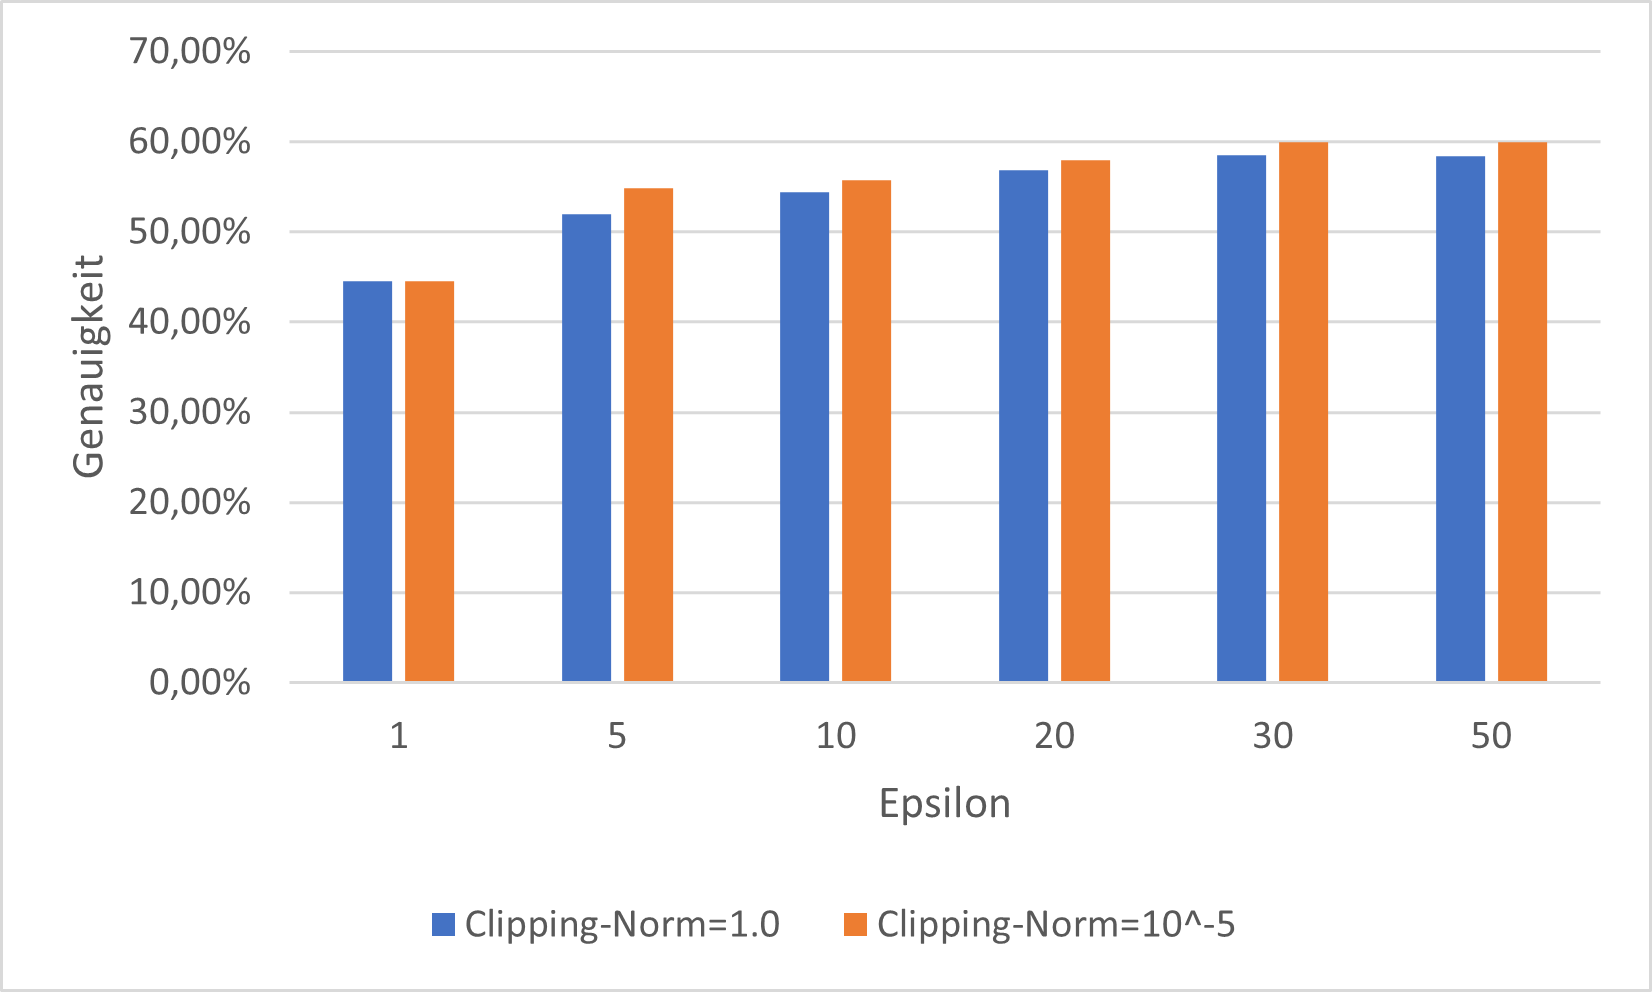
\includegraphics[width=14cm]{figures/results_cifar/cifar_clipp2.png}
    \caption{Auswirkung der Clipping-Norm auf die Güte von CIFAR-10 Modellen bei 30 Epochen Training}
    \label{fig:cifar_clip2}
\end{figure} 


Für das CIFAR-10 Modell mit DPSGD resultieren folgende Hyperparameter in einer optimalen Güte des Modells:
\begin{compactitem}
    \item \textbf{$\epsilon$-Wert des Privacy Budgets:} Der $\epsilon$-Wert korreliert mit der Güte des Modells. Kleine Werte schränken die Genauigkeit der Modelle ein, können aber die Vertraulichkeit besser schützen. Kapitel \ref{sec:bw_dp} gibt dabei einen Überblick über den Schutz der Modelle.
    \item \textbf{Batch-Größe:} Die Batch-Größe sollte möglichst groß gewählt werden. Hier kann ebenfalls der BatchMemoryManager von Opacus helfen, welcher eine virtuelle Batch-Größe ermöglicht, ohne den Speicher zu überlasten. Eine Batch-Größe von 512 bietet jedoch keinen Vorteil mehr gegenüber einer Batch-Größe von 256.
    \item \textbf{Anzahl Epochen:} Die Anzahl an Epochen ist höher als bei einem Modell ohne DPSGD. 
    Dies liegt daran, dass das Rauschen Overfitting abschwächt. Wird ein geringer Wert für die Clipping-Norm gewählt, können sogar noch mehr Epochen trainiert werden.
    Eine Epochenanzahl von 30 bietet immer noch eine steigende Genauigkeit, wohingegen ein Modell ohne DPSGD bereits nach 15 Epochen stagniert.
    \item \textbf{Datenaugmentierung:} Datenaugmentierung ist nicht notwendig und kann die Güte des Modells sogar verschlechtern.
    \item \textbf{Clipping-Norm:} Der Wert der Clipping-Norm sollte möglichst gering gewählt werden. Dies ermöglicht das Training von mehreren Epochen, wobei das Rauschen verringert wird.
\end{compactitem}

Tabelle \ref{tab:c10_dpsgd_res} zeigt, welche Genauigkeit mit verschiedenen $\epsilon$-Werten erreicht wird, wenn die Hyperparameter nach obigen Regeln optimiert werden.
\begin{table}[!htb]
\centering
\begin{tabular}{|l|l|l|l|l|}
\hline
\rowcolor[HTML]{CBCEFB} 
Epsilon  & \begin{tabular}[c]{@{}l@{}}Anzahl\\ Epochen\end{tabular} & Batch-Größe &Clipping-Norm & Genauigkeit \\ \hline

1  & 30 & 512 & $10^{-5}$  & 46,7 \% \\ \hline
5  & 30 & 512 & $10^{-5}$  & 55,0 \% \\ \hline
10 & 30 & 512 & $10^{-5}$  & 59,4 \% \\ \hline
20 & 30 & 512 & $10^{-5}$  & 60,5 \% \\ \hline
30 & 30 & 512 & $10^{-5}$  & 61,9 \% \\ \hline
50 & 30 & 512 & $10^{-5}$  & 63,2 \% \\ \hline
\end{tabular}
\caption{Genauigkeit von CIFAR-10 Modellen mit DPSGD}
\label{tab:c10_dpsgd_res}
\end{table}

\subsection{Hyperparameter ResNet-18 Modell}

Das originale ResNet-18 Modell ist für die Klassifikation des ImageNet Datenbestands trainiert. 
Da das Modell jedoch dafür genutzt werden soll, Merkmale aus Gesichtsbildern der CelebA Datenmenge zu erkennen, wird das Modell angepasst.
Dafür wird die ursprünglich letzte, vollständig verbundene Schicht durch eine neue, vollständig verbundene Schicht ausgetauscht, welche nur 40 Neuronen enthält.
Jedes Neuron steht dabei für eines der Merkmale.

Das ResNet-18 Modell bietet die Möglichkeit, die vortrainierten Gewichte zu nutzen, oder die Gewichte zufällig zu initialisieren.
Deshalb wird der Parameter \dq Vortrainiert\dq\ als zusätzlicher Hyperparameter evaluiert.
Dabei ist anzumerken, dass das Modell mit dem ImageNet Datenbestand vortrainiert ist, welches Bilder von Objekten enthält, jedoch nicht primär von Gesichtern.

Das vortrainierte ResNet-18 Modell ohne DPSGD erreicht eine Genauigkeit von 92,4 \% nach 10 Epochen mit Datenaugmentierung.
Wird stattdessen das nicht-vortrainierte Modell genommen, liegt die Genauigkeit bei 92,3 \%, also minimal darunter.
Das Deaktivieren der Datenaugmentierung hat jedoch einen größeren negativen Einfluss. 
Dadurch würde die Güte des Modells auf 91,0 \% für das vortrainierte und auf 90,1 \% für das nicht-vortrainierte Modell sinken.

Die Auswirkung der Hyperparameter des ResNet-18 Modells mit DPSGD ist gleich wie bei dem CIFAR-10 Modell.
Höhere Batch-Größen, eine niedrige Clipping-Norm und keine Nutzung von Datenaugmentierung sorgen für eine Verbesserung der Genauigkeit des Modells. 
Ob das Modell dabei vortrainiert oder nicht-vortrainiert ist, spielt eine untergeordnete Rolle und wirkt sich kaum auf die Genauigkeit der Modelle aus.
Anhang \ref{ch:ergebnisse_detail} enthält Tabellen mit detaillierten Messungen zu verschiedenen Hyperparametern von DPSGD.
Im Folgenden werden nur die besten Modelle betrachtet.

\begin{table}[!htb]
\centering
\begin{tabular}{|l|l|l|l|l|l|}
\hline
\rowcolor[HTML]{CBCEFB} 
Epsilon  & Clipping-Norm & Batch-Größe & \begin{tabular}[c]{@{}l@{}}Anzahl\\ Epochen\end{tabular} & \begin{tabular}[c]{@{}l@{}}Daten-\\ augmentierung\end{tabular} & Genauigkeit \\ \hline
$\infty$ & $\infty$      & 128         & 10                                                       & ja                                                             & 92,3 \%     \\ \hline
1        & $10^{-5}$     & 256         & 10                                                       & nein                                                           & 83,6 \%     \\ \hline
5        & $10^{-5}$      & 256         & 10                                                       & nein                                                           & 86,4 \%     \\ \hline
10       & $10^{-5}$     & 256         & 10                                                       & nein                                                           & 86,8 \%     \\ \hline
\end{tabular}
\caption{Übersicht der besten ResNet-18 Modelle mit DPSGD}
\label{tab:r18_best}
\end{table}

Tabelle \ref{tab:r18_best} zeigt dabei, was für eine Genauigkeit von Modellen erreicht werden kann, abhängig von unterschiedlichen $\epsilon$-Werten.
Die virtuelle Batch-Größe ist bei den DPSGD Modellen auf 256 gesetzt, wohingegen die physische Batch-Größe bei 64 liegt.
Der Wert für das Clipping wird auf $10^{-5}$ gesetzt, welcher einen leicht negativen Einfluss auf das Modell hat, bei einem $\epsilon$-Wert von unendlich.
Datenaugmentierung verschlechtert die Güte des Modells bei der Nutzung von DPSGD, weshalb diese nicht genutzt wird.
Bei einem $\epsilon$-Wert von 1 erreicht das Modell eine Genauigkeit von 83,6 \% und liegt damit absolut 8,7 \% unter dem Modell ohne DPSGD. 
Wird der $\epsilon$-Wert auf 10 erhöht, steigt die Genauigkeit auf 86,8 \% an. 
Damit hat dieses Modell nur 5,5 Prozentpunkte weniger Genauigkeit, als das Modell ohne DPSGD.

\subsection{Hyperparameter Vision Transformer Modell}

Das Vision Transformer Modell in PyTorch ist standardmäßig ebenfalls für die ImageNet-Datenmenge vortrainiert.
Dies bedeutet, dass hier ebenfalls die letzte, vollständig verbundene Schicht ausgetauscht wird, mit einer Schicht, welche 40 Neuronen, ein Neuron pro Merkmal, enthält.

Das vortrainierte Vision Transformer Modell ohne DPSGD erreicht eine Genauigkeit von 82,9 \% nach 10 Epochen mit Datenaugmentierung. 
Ohne Datenaugmentierung liegt die Genauigkeit bei 83,0 \% und damit minimal höher als mit Datenaugmentierung.
Wird jedoch das nicht-vortrainierte Vision Transformer Modell genutzt, sinken die Genauigkeiten auf 82,4 \% für das Modell ohne Datenaugmentierung und 82,3 \% für das Modell mit Datenaugmentierung.
Dies lässt schlussfolgern, dass die Nutzung von Datenaugmentierung kaum Einfluss auf das Modell ohne DPSGD hat.
Außerdem wird deutlich, dass das Vision Transformer Modell schlechter geeignet ist für die Merkmalserkennung aus Gesichtern, als das ResNet-18 Modell.

\begin{table}[!htb]
\centering
\begin{tabular}{llllll}
\hline
\rowcolor[HTML]{CBCEFB} 
\multicolumn{1}{|l|}{\cellcolor[HTML]{CBCEFB}Epsilon} & \multicolumn{1}{l|}{\cellcolor[HTML]{CBCEFB}Clipping-Norm} & \multicolumn{1}{l|}{\cellcolor[HTML]{CBCEFB}Batch-Größe} & \multicolumn{1}{l|}{\cellcolor[HTML]{CBCEFB}\begin{tabular}[c]{@{}l@{}}Anzahl\\ Epochen\end{tabular}} & \multicolumn{1}{l|}{\cellcolor[HTML]{CBCEFB}\begin{tabular}[c]{@{}l@{}}Daten-\\ augmentierung\end{tabular}} & \multicolumn{1}{l|}{\cellcolor[HTML]{CBCEFB}Genauigkeit} \\ \hline
\multicolumn{1}{|l|}{1}                               & \multicolumn{1}{l|}{1,0}                                   & \multicolumn{1}{l|}{16}                                  & \multicolumn{1}{l|}{5}                                                                                & \multicolumn{1}{l|}{ja}                                                                                     & \multicolumn{1}{l|}{79,4 \%}                             \\ \hline
\multicolumn{1}{|l|}{1}                               & \multicolumn{1}{l|}{$10^{-5}$}                             & \multicolumn{1}{l|}{128}                                 & \multicolumn{1}{l|}{5}                                                                                & \multicolumn{1}{l|}{nein}                                                                                   & \multicolumn{1}{l|}{80,0 \%}                             \\ \hline
                                                      &                                                            &                                                          &                                                                                                       &                                                                                                             &                                                          \\ \hline
\multicolumn{1}{|l|}{5}                               & \multicolumn{1}{l|}{1,0}                                   & \multicolumn{1}{l|}{16}                                  & \multicolumn{1}{l|}{5}                                                                                & \multicolumn{1}{l|}{ja}                                                                                     & \multicolumn{1}{l|}{78,8 \%}                             \\ \hline
\multicolumn{1}{|l|}{5}                               & \multicolumn{1}{l|}{$10^{-5}$}                             & \multicolumn{1}{l|}{128}                                 & \multicolumn{1}{l|}{5}                                                                                & \multicolumn{1}{l|}{nein}                                                                                   & \multicolumn{1}{l|}{80,0 \%}                             \\ \hline
                                                      &                                                            &                                                          &                                                                                                       &                                                                                                             &                                                          \\ \hline
\multicolumn{1}{|l|}{10}                              & \multicolumn{1}{l|}{1,0}                                   & \multicolumn{1}{l|}{16}                                  & \multicolumn{1}{l|}{5}                                                                                & \multicolumn{1}{l|}{ja}                                                                                     & \multicolumn{1}{l|}{79,4 \%}                             \\ \hline
\multicolumn{1}{|l|}{10}                              & \multicolumn{1}{l|}{$10^{-5}$}                             & \multicolumn{1}{l|}{128}                                 & \multicolumn{1}{l|}{5}                                                                                & \multicolumn{1}{l|}{nein}                                                                                   & \multicolumn{1}{l|}{80,3 \%}                             \\ \hline
\end{tabular}
\caption{Vergleich der Hyperparameter bei Vision Transformer Modellen}
\label{tab:vit_comp1}
\end{table}

Die Wahl der Hyperparameter hat außerdem bei diesem Modell weniger Einfluss auf die Genauigkeit, als bei den beiden vorherigen Modellen.
Tabelle \ref{tab:vit_comp1} zeigt, welche Genauigkeit die Vision Transformer Modelle mit DPSGD erreichen, wenn die Hyperparameter optimiert werden.
Dabei wird jeweils das vortrainierte Vision Transformer Modell genutzt.
Die unoptimierten Hyperparameter sind dabei eine Batch-Größe von 16, Nutzung von Datenaugmentierung und eine Clipping-Norm von 1,0.
Das Optimieren der Parameter erhöht die Batch-Größe auf 128, reduziert die Clipping-Norm auf $10^{-5}$ und deaktiviert die Nutzung von Datenaugmentierung.
Zusätzlich ist anzumerken, dass die DPSGD Modelle maximal für 5 Epochen trainiert wurden. 
Dies liegt daran, dass eine Epoche \ca 50 Minuten Zeit benötigt, was die Evaluierungsmöglichkeiten einschränkt.
Zudem gibt es keine signifikante Verbesserung der Genauigkeit bei einem Training des Vision Transformer Modells mit DPSGD von 3 Epochen und 5 Epochen.
Dies lässt andeuten, dass es ebenfalls keine signifikante Verbesserung der Genauigkeit bei 5 Epochen und 10 Epochen gibt.
Das Optimieren der Hyperparameter sorgt für eine absolute Verbesserung der Genauigkeit von 0,6, 1,2 und 0,8 Prozentpunkte, je nach Wahl von $\epsilon$.

\begin{table}[!htb]
\centering
\begin{tabular}{|l|l|l|l|l|l|}
\hline
\rowcolor[HTML]{CBCEFB} 
Epsilon  & Clipping-Norm & Batch-Größe & \begin{tabular}[c]{@{}l@{}}Anzahl\\ Epochen\end{tabular} & \begin{tabular}[c]{@{}l@{}}Daten-\\ augmentierung\end{tabular} & Genauigkeit \\ \hline
$\infty$ & $\infty$      & 64          & 10 & nein & 83,0 \%     \\ \hline
1        & $10^{-5}$     & 128         & 5 & nein & 80,0 \%     \\ \hline
5        & $10^{-5}$     & 128         & 5 & nein  & 80,0 \%     \\ \hline
10       & $10^{-5}$     & 128         & 5 & nein  & 80,3 \%     \\ \hline
\end{tabular}
\caption{Übersicht der besten Vision Transformer Modelle mit DPSGD}
\label{tab:vit_best}
\end{table}
Tabelle \ref{tab:vit_best} stellt die Genauigkeit des besten Vision Transformer Modells ohne DPSGD in Relation zu den Genauigkeiten der Vision Transformer Modelle mit DPSGD und optimierten Hyperparametern.
Die Genauigkeit des Modells ohne DPSGD ist bis zu 3 Prozentpunkte höher, als bei den Modellen mit DPSGD. 
Damit fällt Differenz der Genauigkeit von Modellen ohne DPSGD und mit DPSGD geringer aus, als bei den beiden vorherigen Modellarten.

\subsection{Handlungsempfehlung für die Wahl der Hyperparameter}

Die folgende Handlungsempfehlung zeigt, wie die Hyperparameter optimiert werden müssen, um die bestmögliche Güte eines Modells mit DPSGD zu erhalten. 
Der $\epsilon$-Wert wird hierbei außer Betracht gelassen.
Datenaugmentierung gilt es ebenfalls zu vermeiden.

\subsubsection*{Batch-Größe}
Da das Training mit DPSGD von Opacus mehr Speicher als das gleiche Training ohne DPSGD benötigt, muss zuerst eine geeignete Batch-Größe herausgefunden werden.
Dabei gibt es eine physische Batch-Größe, die Batch-Größe, die wirklich gleichzeitig in den Speicher passt, und eine virtuelle Batch-Größe, die größer sein kann.
Um die physische Batch-Größe zu finden, müssen die entsprechenden PyTorch Klassen in die Opacus Wrapper-Klassen eingebunden werden.
Die Parameter \bzgl dem Rauschen und Clipping können dabei ignoriert werden.
Anschließend kann ein Batch genutzt werden, um die Gradienten zu berechnen. 
An dieser Stelle ist es möglich, den Speicherverbrauch zu überwachen und so lange die Batch-Größe anzupassen, bis der Speicher optimal ausgenutzt ist.
Die virtuelle Batch-Größe kann größer gewählt werden, als die physische Batch-Größe.
Eine relativ große Batch-Größe sorgt dafür, dass die Werte des Rauschens sich ausgleichen. 
Eine zu große Batch-Größe hat jedoch auch negative Folgen.
Es empfiehlt sich eine Batch-Größe von 128, 256 oder 512.

\subsubsection*{Anzahl der Epochen}
Um die Stärke des Rauschens zu setzen, ist es wichtig, die geplante Anzahl an Epochen im Voraus zu kennen.
Die Anzahl der Epochen, welche bei einem Training mit DPSGD benötigt werden, können von dem Modell ohne DPSGD abgleitet werden.
Da das Hinzufügen von Rauschen als eine Art Regularisierung betrachtet werden kann, wird Overfitting durch DPSGD vermieden.
Somit könnten einige Epochen mehr trainiert werden, als bei dem Modell ohne DPSGD.
Die Evaluierung des ResNet-18 Modells und des Vision Transformer Modells haben jedoch kaum Verbesserungen bei einer hohen Anzahl an Epochen gezeigt.
Ein guter Richtwert ist es also, dass das Modell mit DPSGD für die gleiche Anzahl an Epochen trainiert wird, wie das Modell ohne DPSGD.

\subsubsection*{Clipping-Norm}
Der Wert des Clippings hat direkten Einfluss auf die Stärke des Rauschens und sollte deshalb klein gesetzt werden.
Ist der Wert jedoch zu klein, werden die Gradienten ebenfalls zu klein und das Modell wird nicht konvergieren.
Um eine ideale Clipping-Norm zu ermitteln, kann ein Modell für eine kleine Anzahl an Epochen mit DPSGD und Opacus trainiert werden. 
Der Wert des Rauschens wird dabei auf 0 gesetzt, wodurch sich ein $\epsilon$-Wert von unendlich ergibt.
Anschließend werden mehrere Modelle trainiert, welche jeweils eine unterschiedliche Zehnerpotenz als Clipping-Norm haben.
Die Clipping-Norm wird jeweils um eine Zehnerpotenz reduziert, solange bis ein Modell eine signifikant schlechtere Güte zeigt.
Dies bedeutet, dass diese Zehnerpotenz als Clipping-Norm eine signifikante Menge an Gradienten begrenzt und somit ein geeigneter Wert ist.


\section{Angriffe}\label{sec:exp_angriffe}

Das Ziel von Differential Privacy in Kombination mit neuronalen Netzen, ist es, Angriffe abzuschwächen. 
Im Folgenden wird anhand zweier Angriffe evaluiert, welchen Effekt die Nutzung von DPSGD hat.
Bei den zwei genutzten Angriffen handelt es sich um die Membership Inference Attacke und die Model Inversion Attacke.

\subsection{Membership Inference Attacke}

Die Membership Inference Attacke soll zeigen, ob ein Datensatz in der Trainingsdatenmenge eines Modells enthalten ist oder nicht.
Dazu werden Shadow Modelle genutzt, welche das anzugreifende Modell nachahmen. 
Die Vorhersagen der Shadow Modelle werden genutzt, um einen Meta-Klassifikator zu trainieren, welcher bestimmt, ob ein Datensatz bei einem Modell zum Training genutzt wurde.

Eine Besonderheit dieses Angriffs ist es, dass sowohl eine Black-Box, als auch eine White-Box Variante möglich ist.
Bei der White-Box Variante kennt der Angreifer die genaue Architektur des anzugreifenden Modells und kann die Architektur der Shadow Modell nachbilden.
In der Black-Box Variante, wird lediglich versucht, ähnliche Architekturen zu kreieren.
Dieses Experiment nutzt den White-Box Ansatz.
Dies liegt daran, dass es bei einem Black-Box Ansatz sein könnte, dass der Angreifer, durch Glück, eine nahezu identische Architektur der Shadow Modelle wählt. 
Somit kann ein Black-Box Ansatz theoretisch genauso effektiv sein, wie der White-Box Ansatz.

\subsubsection*{Membership Inference Attacke gegen das CIFAR-10 Modell}

Die CIFAR-10 Datenmenge besteht bereits aus einer Trainingsdatenmenge und einer Testdatenmenge, welche in Summe aus 60000 Datensätzen bestehen.
Für das Training der Shadow Modelle werden die beiden Datenmengen kombiniert.
Anschließend wird für jedes Shadow Modell zufällig eine Datenmenge, bestehend aus 50000 Datensätzen, für das Training ausgewählt.
Somit dienen die ausgewählten Daten nicht nur für das Training, sondern haben zusätzlich das Label \dq included\dq, wohingegen die nicht ausgewählten Daten das Label \dq excluded\dq\ erhalten.
Die Labels dienen im Anschluss dazu, die Datenmenge für den Meta-Klassifikator zu konstruieren.
Damit die Anzahl der beiden Labels in der Datenmenge gleich ist, werden von der genutzten Trainingsdatenmenge jedes Shadow Modells nur 10000 Datensätze gelabelt.
Somit entstehen pro Shadow Modell 20000 gelabelte Datensätze, jeweils 10000 mit dem Label \dq included\dq\ und 10000 mit dem Label \dq excluded\dq.

Der Meta-Klassifikator ist ein neuronales Netz, welches nur aus vollständig verbundenen Schichten besteht.
Dabei werden 10 Neuronen als Eingabe genutzt, je ein Neuron pro Vorhersagewahrscheinlichkeit einer Klasse, und ein Neuron als Ausgabe, welches das Label \dq included\dq\ oder \dq excluded\dq\ bestimmt.
Die Vorhersagewahrscheinlichkeiten, welche als Eingabe dienen, werden von den Shadow Modellen durch die Softmax-Funktion in den Wertebereich (0,1) übertragen, wobei eine Klasse einen Wert nahe 1 hat, die restlichen Klassen einen Wert von 0.

Die Trainingsdatenmenge und Testdatenmenge des CIFAR-10 Datenbestands könnte genutzt werden, um die Membership Inference Attacke zu bewerten, jedoch haben die Datenmengen eine ungleiche Anzahl an Datensätzen.
Würde der Meta-Klassifikator immer das Label \dq included\dq\ bestimmen, unabhängig des Inputs, dann entspräche dies einer Genauigkeit von \ca 83,3 \%, da die Anzahl der Datensätze in den beiden Datenmengen das gleiche Verhältnis haben.
Deshalb werden aus der Trainingsdatenmenge zufällig 10000 Datensätze ausgewählt. Diese, sowie die 10000 Datensätze der Testdatenmenge, dienen dann zur Evaluierung des Angriffs.
Dazu werden die Datensätze durch das anzugreifende Modell inferiert und die Vorhersagewahrscheinlichkeiten als Eingabe des Meta-Klassifikators genutzt.

Die Modelle, an welchen die Membership Inference Attacke getestet wird, sind die Modelle, welche in Kapitel \ref{sec:hyperparams} trainiert werden.
Dabei wird das beste Modell ohne DPSGD genutzt, sowie jeweils das Modell mit DPSGD, welches mit optimierten Hyperparametern trainiert wurde.

Tabelle \ref{tab:mi_cifar10_base} zeigt die Genauigkeit, welche der Meta-Klassifikator bei der Ausführung der Membership Inference Attacke gegen das CIFAR-10 Modell ohne DPSGD hat.
Dabei wurden eine unterschiedliche Anzahl an Shadow Modellen evaluiert, welche jeweils für 15 Epochen trainiert wurden und dadurch eine ähnliche Genauigkeit wie das originale Modell haben.
Die Genauigkeit des Angriffs ist bei 8,16 und 32 Shadow Modellen ähnlich.
Diese beträgt zwischen 57,4 \% und 58,9 \%.
\begin{table}[!htb]
\centering
\begin{tabular}{|l|l|l|}
\hline
\rowcolor[HTML]{CBCEFB} 
Epsilon & Anzahl Shadow Modelle & Genauigkeit des Angriff \\ \hline
$\infty$ & 8  & 58,0 \% \\ \hline
$\infty$ & 16 & 58,9 \% \\ \hline
$\infty$ & 32 & 57,4 \% \\ \hline
\end{tabular}
\caption{Membership Inference Angriff gegen CIFAR-10 Modell ohne DPSGD}
\label{tab:mi_cifar10_base}
\end{table}

Tabelle \ref{tab:mi_cifar10_part1} zeigt, wie sich die Genauigkeit des Angriffs durch die Nutzung von DPSGD ändert.
Bei allen Modellen mit DPSGD, hat die Membership Inference Attacke eine Genauigkeit zwischen 49,8 \% und 50,2 \%. 
Dadurch ist der Angriff weniger effektiv, als ohne die Nutzung von DPSGD.
\begin{table}[!htb]
\centering
\begin{tabular}{|l|l|l|}
\hline
\rowcolor[HTML]{CBCEFB} 
Epsilon & \begin{tabular}[c]{@{}l@{}}Anzahl \\ Shadow Modelle\end{tabular} & \begin{tabular}[c]{@{}l@{}}Genauigkeit \\ des Angriff\end{tabular} \\ \hline
$\infty$ & 32 & 57,4 \% \\ \hline
1        & 32 & 49,9 \% \\ \hline
5        & 32 & 49,8 \% \\ \hline
10       & 32 & 50,1 \% \\ \hline
20       & 32 & 50,2 \% \\ \hline
30       & 32 & 50,2 \% \\ \hline
50       & 32 & 50,0 \% \\ \hline
\end{tabular}
\caption{Membership Inference Angriff gegen CIFAR-10 Modelle mit DPSGD}
\label{tab:mi_cifar10_part1}
\end{table}

Das Problem des Angriffs ist jedoch, dass dieser nur minimal effektiv gegen ein Modell ohne DPSGD ist. 
Würde der Meta-Klassifikator zufällig ein Label wählen, würde dies einer Genauigkeit von \ca 50 \% entsprechen. 
Gegen ein Modell ohne DPSGD, erreicht der Meta-Klassifkator eine Genauigkeit von bis zu 58,9 \%, was eine Verbesserung ist.
Jedoch ermöglicht dies nicht, eine sachdienliche Aussage zu treffen.
Zusätzlich hat der Angreifer in der Regel keine Möglichkeit, den Angriff zu evaluieren. 
Dies liegt daran, dass der Angreifer keine Informationen \bzgl der genutzten Trainingsdatenmenge hat.
Die geringe Effektivität des Angriffs, sogar in der White-Box Variante, macht die Nutzung von DPSGD entbehrlich.

\subsubsection*{Membership Inference Attacke gegen das ResNet-18 Modell}
Die Membership Inference Attacke wird nur gegen das ResNet-18 Modell evaluiert, jedoch nicht gegen das Vision Transformer Modell.
Dies liegt an den benötigten Ressourcen, eine Vielzahl an Shadow Modellen zu trainieren, welche jeweils die Vision Transformer Architektur nutzen.

Das ResNet-18 Modell erkennt 40 Merkmale anhand von Gesichtsbildern des CelebA Datenbestand.
Im Gegensatz zu dem CIFAR-10 Modell wird nicht eine Klasse vorhergesagt, sondern 40 unabhängige Merkmale.
Dabei handelt es sich um eine sogenannte Multi-Label Klassifizierung, also einer Klassifikation bei welcher mehrere Labels vorhergesagt werden können.
Für das Modell sind diese 40 Labels unabhängig, fachlich sind jedoch einige dieser Labels verbunden.
So gibt es beispielsweise unterschiedliche Labels, welche für unterschiedliche Haarfarben stehen.
Da jede Person in dem Datenbestand eine Haarfarbe hat, hat maximal eines der Haarfarben-Labels den Wert 1, wohingegen die restlichen Haarfarben den Wert 0 haben.

Die Membership Inference Attacke gegen die ResNet-18 Modelle werden simultan zu den Angriffen gegen die CIFAR-10 Modelle durchgeführt.
Tabelle \ref{tab:mi_resnet18} zeigt die Genauigkeit des Angriffs gegen Modelle mit einem unterschiedlichen $\epsilon$-Wert.
Es wurden jeweils 8 Shadow Modelle trainiert und zum Labeln genutzt.
Der Angriff gegen das Modell ohne DPSGD hat eine Genauigkeit von 52,1 \% und ist damit nur minimal besser, als bei einer zufälligen Vorhersage.
Gegen Modelle die DPSGD benutzten ist der Angriff noch weniger effektiv und erreicht eine Genauigkeit von maximal 50,6 \%.

\begin{table}[!htb]
\centering
\begin{tabular}{|l|l|}
\hline
\rowcolor[HTML]{CBCEFB} 
Epsilon  & Genauigkeit des Angriff \\ \hline
$\infty$ & 52,1 \%                 \\ \hline
1        & 50,2 \%                 \\ \hline
5        & 50,6 \%                 \\ \hline
10       & 50,1 \%                 \\ \hline
\end{tabular}
\caption{Membership Inference Angriff gegen ResNet-18 Modelle mit DPSGD}
\label{tab:mi_resnet18}
\end{table}

\subsection{Model Inversion Attacke}

Bei der Model Inversion Attacke werden die Ausgaben eines Modells genutzt, um Rückschlüsse zu den Trainingsdaten zu ziehen.
Der hier evaluierte Angriff wird auch Reconstruction Attacke genannt. 
Ziel ist es, einen Datensatz aus dem Trainingsdatenbestand nachzubilden, lediglich anhand des Modells.
Hierfür wird ein Startbild in das Modell gegeben, welches zu Beginn lediglich eine Ansammlung von zufälligen Pixeln ist.
Die Vorhersage des Modells wird anschließend mit einer Verlustfunktion durch das Modell backpropagiert, jedoch werden nicht die Gewichte des Modells angepasst, sondern die Werte des Startbildes.
Dadurch verändert sich das Bild, bis es das gewünschte Label zeigt.
Der Vorgang wird dabei iterativ wiederholt.
Zusätzlich wird in jedem Schritt das Bild mittels eines Autoencoders entrauscht, sodass sich die zufällige Ansammlung von Pixeln zu einem möglichst realistischen Bild umwandeln.
Der iterative Vorgang kann nach einer festgelegten Anzahl an Wiederholungen gestoppt werden, oder bis das rekonstruierte Bild den gewünschten Detailgrad erreicht hat.

\subsubsection*{Model Inversion Attacke gegen CIFAR-10 Modell}
Um die Model Inversion Attacke durchzuführen, wurde zu Beginn ein Autoencoder trainiert.
Dieser soll Bilder entrauschen, \dahe das Rauschen aus Bildern entfernen und diese realistischer werden lassen.
Als Ausgabe des Modells werden daher die Bilder des CIFAR-10 Trainingsdatenbestand genutzt, wobei die Eingabe jeweils eine verrauschte Version dieses Bildes ist.
Die verrauschten Bilder können erzeugt werden, indem ein zufälliges Rauschen über jedes Pixel hinzugefügt wird.

Der Autoencoder hat die gleiche Eingabedimension wie Ausgabedimension, welche $32\times32\times3$ Pixeln entspricht.
In einer verdeckten Schicht ist die Dimension jedoch niedriger, welche dafür sorgt, dass das Modell in dieser nur einen Teil der Bildinformationen zwischenspeichern kann.
Zum Verkleinern der Dimensionen werden Faltungsschichten und Pooling-Operationen genutzt.
Das Vergrößern der Dimension wird mit transponierten Faltungsschichten ausgeführt.
Transponierte Faltungsschichten funktionieren simultan zu normalen Faltungsschichten, jedoch wird zuvor das Bild um interpolierte Pixel erweitert. 
Abbildung \ref{fig:autoencoder_cifar} zeigt, welchen Effekt der Autoencoder auf verrauschte Bilder ausübt.
Der linke Teil der Abbildung zeigt ein originales Bild aus der CIFAR-10 Datenmenge. 
Dieses ist der Klasse \dq Schiff\dq\ untergeordnet.
Der mittlere Teil der Abbildung zeigt dabei die zufällig verrauschte Version dieses Bildes.
Das Schiff ist dabei kaum zu erkennen, da viele Pixel des Bildes eine andere Farbe angenommen haben.
Der rechte Teil der Abbildung zeigt, wie die Ausgabe des Autoencoders bei Eingabe des verrauschten Bildes aussieht.
Das Schiff ist wieder erkennbar und das Bild ähnelt dem originalen Bild.

\begin{figure}[!htb]
\centering
\begin{subfigure}[h]{0.3\textwidth}
  \centering
  
\includegraphics[width=\linewidth]{figures/autoencoder_cifar/1.jpg}
  \caption{Originales Bild}
\end{subfigure}
\begin{subfigure}[h]{0.3\textwidth}
  \centering
  
\includegraphics[width=\linewidth]{figures/autoencoder_cifar/2.jpg}
  \caption{Verrauschtes Bild}
\end{subfigure}
\begin{subfigure}[h]{0.3\textwidth}
  \centering
  
\includegraphics[width=\linewidth]{figures/autoencoder_cifar/3.jpg}
  \caption{Ausgabe Autoencoder}
\end{subfigure}
\caption{Autoencoder CIFAR-10 Datenbestand}
\label{fig:autoencoder_cifar}
\end{figure}

Wird die Model Inversion Attacke gegen das CIFAR-10 Modell ohne DPSGD ausgeführt, kann kein Bild rekonstruiert werden.
Parameter wie der Optimizer, die Lernrate oder die Verlustfunktion wurden angepasst, jedoch führte dies zu keiner Verbesserung des Angriffs 
Zusätzlich wurden unterschiedliche Methoden der Initialisierung des Startbildes gewählt.
Ebenfalls wurden evaluiert, den Angriff einige Iterationen ohne den Autoencoder durchzuführen.
Keine der Anpassungen sorgte für eine Verbesserung des Angriffs.

Abbildung \ref{fig:moder_inv_c10} zeigt, das Ergebnis einer Model Inversion Attacke, wenn ein Bild mit dem Label \dq Schiff\dq\ nachgebildet werden soll.
Das linke Bild entspricht dem initialen Startbild, bei dem alle Farbwerte jeweils mit dem Wert 0,5 befüllt werden. 
Dies entspricht einem grauen Bild.
Das mittlere Bild zeigt, wie sich das Bild nach einigen Iterationen des Angriffs ohne Autoencoder verändert hat.
Dabei handelt es sich um zufällig aussehende Pixel, jedoch sagt das CIFAR-10 Modell bei diesem Bild das gewünschte Label \dq Schiff\dq\ vorher.
Das rechte Bild zeigt das Ergebnis des Angriffs, nachdem das Bild für weitere Iterationen angepasst wurde und pro Iteration mit dem Autoencoder angepasst wurde.
Das entstandene Bild besteht primär aus gräulichen Pixeln, welche eine Musterung aufweisen, die vermutlich vom Autoencoder stammt.
Es ist kein Schiff zu erkennen.
\begin{figure}[!htb]
\centering
\begin{subfigure}[h]{0.3\textwidth}
  \centering
  
\includegraphics[width=\linewidth]{figures/autoencoder_cifar/mi_cifar_start_grey.jpg}
  \caption{Initiales Bild\\jeder Wert=0,5}
\end{subfigure}
\begin{subfigure}[h]{0.3\textwidth}
  \centering
  
\includegraphics[width=\linewidth]{figures/autoencoder_cifar/mi_cifar_mid_grey.jpg}
  \caption{Anpassung \\ohne Autoencoder}
\end{subfigure}
\begin{subfigure}[h]{0.3\textwidth}
  \centering
  
\includegraphics[width=\linewidth]{figures/autoencoder_cifar/mi_cifar_finish_grey.png}
  \caption{Anpassung \\mit Autoencoder}
\end{subfigure}
\caption{Model Inversion Attacke gegen CIFAR-10}
\label{fig:moder_inv_c10}
\end{figure}

\subsubsection*{Model Inversion Attacke gegen ResNet-18 Modell}

Die Model Inversion Attacke gegen das ResNet-18 Modell erfolgt simultan zu der Attacke gegen das CIFAR-10 Modell.
Zuerst wird ein Autoencoder trainiert, welcher das Rauschen von Bildern der CelebA Datenmenge entfernt.
Abbildung \ref{fig:autoencoder_celeba} zeigt, wie ein verrauschtes Bild mittels des Autoencoders wieder entrauscht werden kann.
Der Output des Autoencoders, also das entrauschte Bild, zeigt das Gesicht einer Person, jedoch ist das Bild weniger scharf als das originale Bild.

\begin{figure}[!htb]
\centering
\begin{subfigure}[h]{0.3\textwidth}
  \centering
  
\includegraphics[width=\linewidth]{figures/autoencoder_r18/faces_autoencoder1.jpg}
  \caption{Originales Bild}
\end{subfigure}
\begin{subfigure}[h]{0.3\textwidth}
  \centering
  
\includegraphics[width=\linewidth]{figures/autoencoder_r18/faces_autoencoder2.jpg}
  \caption{Verrauschtes Bild}
\end{subfigure}
\begin{subfigure}[h]{0.3\textwidth}
  \centering
  
\includegraphics[width=\linewidth]{figures/autoencoder_r18/faces_autoencoder3.jpg}
  \caption{Ausgabe Autoencoder}
\end{subfigure}
\caption{Autoencoder CelebA Datenbestand}
\label{fig:autoencoder_celeba}
\end{figure}

Die Model Inversion Attacke ist ebenfalls gegen das ResNet-18 Modell ohne DPSGD nicht effektiv.
Abbildung \ref{fig:moder_inv_cr18} zeigt dabei das Ergebnis einer Rekonstruktion. 
Die Labels, nach welchen das Bild rekonstruiert werden soll, entstammen dem Beispielbild aus Abbildung \ref{fig:autoencoder_celeba}.
Als Startbild dient hier wieder ein Bild, bei welchem jeder Farbwert auf den Wert 0,5 gesetzt ist.
Dieses wurde für einige Iterationen durch die Backpropagation des Modells angepasst, jedoch vorerst ohne Autoencoder.
Hier entsteht eine zufällige Ansammlung an Pixeln, welche jedoch vom Modell die gewünschten Labels vorhergesagt bekommt.
Nach einigen weiteren Iterationen, sowie zusätzlichen Anpassungen mittels des Autoencoders, entsteht wieder ein relativ gräuliches Bild.
Dieses besitzt ebenfalls eine Musterung, welche vermutlich durch den Autoencoder entstanden ist.
\begin{figure}[!htb]
\centering
\begin{subfigure}[h]{0.3\textwidth}
  \centering
  
\includegraphics[width=\linewidth]{figures/autoencoder_r18/faces_mi1.jpg}
  \caption{Initiales Bild\\jeder Wert=0,5}
\end{subfigure}
\begin{subfigure}[h]{0.3\textwidth}
  \centering
  
\includegraphics[width=\linewidth]{figures/autoencoder_r18/faces_mi2.jpg}
  \caption{Anpassung ohne\\Autoencoder}
\end{subfigure}
\begin{subfigure}[h]{0.3\textwidth}
  \centering
  
\includegraphics[width=\linewidth]{figures/autoencoder_r18/faces_mi3.png}
  \caption{Anpassung mit\\Autoencoder}
\end{subfigure}
\caption{Model Inversion Attacke gegen ResNet-18 Modell}
\label{fig:moder_inv_cr18}
\end{figure}
\section{Zusammenfassung der Experimente}

PyTorch stellt mit Opacus eine Bibliothek zur Verfügung, welche die Nutzung von DPSGD durch einige Wrapper-Klassen ermöglicht.
Opacus bietet über die Klasse \textbf{PrivacyEngine} einen simplen Weg, die PyTorch Objekte entsprechend umzuwandeln. 
Anschließend erfolgt das Training mit normalem PyTorch Code, weshalb die Nutzung von DPSGD mit Opacus kein aufwendiges Refactoring benötigt.
Da jedoch die Funktionsweise von PyTorch durch Opacus angepasst wird, steigt der Speicherverbrauch, sowie die Trainingsdauer einer Epoche (Kaptiel \ref{sec:opacu_implementierung}). 

Durch die richtige Wahl von Hyperparametern kann die Güte von neuronalen Netzen mit DPSGD optimiert werden.
Dazu sollte eine möglichst große Batch-Größe, ein geringer Wert der Clipping-Norm und eine verhältnismäßig hohe Anzahl an Trainingsepochen gewählt werden.
Ein höherer $\epsilon$-Wert sorgt ebenfalls für eine bessere Güte des Modells.
Die Hyperparameter wurden anhand von drei Modellen evaluiert:
\begin{compactitem}
    \item \textbf{CIFAR-10 Modell}: Das CIFAR-10 Modell ist ein neuronales Netz, welches eine ResNet-Architektur mit 10 Schichten nutzt und den CIFAR-10 Datenbestand in 10 unterschiedliche Klassen einteilt. Bei der ResNet-Architektur handelt es sich um ein neuronales Netz mit Faltungsschichten, welches zusätzlich sogenannte Skip Connections nutzt.
    \item \textbf{ResNet-18 Modell}: Das ResNet-18 Modell ist ein neuronales Netz mit 18 Schichten, welches ebenfalls die ResNet-Architektur nutzt. Dieses Modell erkennt 40 Merkmale aus Bildern von menschlichen Gesichtern.
    \item \textbf{Vision Transformer Modell}: Das Vision Transformer Modell erkennt ebenfalls 40 Merkmale aus Bildern von menschlichen Gesichtern.
    Jedoch basiert dieses auf der Transformer-Architektur, welche Embeddings, Aufmerksamkeitsmechanismen und Encoder nutzt.
\end{compactitem}
Die Differenz der Genauigkeit des CIFAR-10 Modells mit DPSGD und ohne DPSGD fällt dabei am größten aus. 
Bei einem $\epsilon$-Wert von 10, sinkt die Genauigkeit von 82,9 \% ohne DPSGD auf eine Genauigkeit von 59,4 \%.
Die Differenz fällt bei dem ResNet-18 Modell und bei dem Vision Transformer Modell geringer aus. 
Bei dem ResNet-18 Modell sinkt die Genauigkeit bei einem $\epsilon$-Wert von 10 um 5,5 Prozentpunkte.
Die Genauigkeit des Vision Transformer Modells sinkt bei einem $\epsilon$-Wert von 10 nur um 2,7 Prozentpunkte (Kapitel \ref{sec:hyperparams}).

Die Wahl von $\epsilon$ und der damit einhergehende Schutz ist abhängig von der benötigten Sicherheit.
Jedoch wird gezeigt, dass die Membership Inference Attacke und die Model Inversion Attacke bei den genutzten Use Cases nicht effektiv ist. 
Sogar bei den Modellen ohne DPSGD sind die Angriffe unwirksam (Kapitel \ref{sec:exp_angriffe}).










